% Latex header for doxygen 1.8.13
\documentclass[twoside]{book}

% Packages required by doxygen
\usepackage{fixltx2e}
\usepackage{calc}
\usepackage{doxygen}
\usepackage[export]{adjustbox} % also loads graphicx
\usepackage{graphicx}
\usepackage[utf8]{inputenc}
\usepackage{makeidx}
\usepackage{multicol}
\usepackage{multirow}
\PassOptionsToPackage{warn}{textcomp}
\usepackage{textcomp}
\usepackage[nointegrals]{wasysym}
\usepackage[table]{xcolor}

% NLS support packages
\usepackage[french]{babel}

% Font selection
\usepackage[T1]{fontenc}
\usepackage[scaled=.90]{helvet}
\usepackage{courier}
\usepackage{amssymb}
\usepackage{sectsty}
\renewcommand{\familydefault}{\sfdefault}
\allsectionsfont{%
  \fontseries{bc}\selectfont%
  \color{darkgray}%
}
\renewcommand{\DoxyLabelFont}{%
  \fontseries{bc}\selectfont%
  \color{darkgray}%
}
\newcommand{\+}{\discretionary{\mbox{\scriptsize$\hookleftarrow$}}{}{}}

% Page & text layout
\usepackage{geometry}
\geometry{%
  a4paper,%
  top=2.5cm,%
  bottom=2.5cm,%
  left=2.5cm,%
  right=2.5cm%
}
\tolerance=750
\hfuzz=15pt
\hbadness=750
\setlength{\emergencystretch}{15pt}
\setlength{\parindent}{0cm}
\setlength{\parskip}{3ex plus 2ex minus 2ex}
\makeatletter
\renewcommand{\paragraph}{%
  \@startsection{paragraph}{4}{0ex}{-1.0ex}{1.0ex}{%
    \normalfont\normalsize\bfseries\SS@parafont%
  }%
}
\renewcommand{\subparagraph}{%
  \@startsection{subparagraph}{5}{0ex}{-1.0ex}{1.0ex}{%
    \normalfont\normalsize\bfseries\SS@subparafont%
  }%
}
\makeatother

% Headers & footers
\usepackage{fancyhdr}
\pagestyle{fancyplain}
\fancyhead[LE]{\fancyplain{}{\bfseries\thepage}}
\fancyhead[CE]{\fancyplain{}{}}
\fancyhead[RE]{\fancyplain{}{\bfseries\leftmark}}
\fancyhead[LO]{\fancyplain{}{\bfseries\rightmark}}
\fancyhead[CO]{\fancyplain{}{}}
\fancyhead[RO]{\fancyplain{}{\bfseries\thepage}}
\fancyfoot[LE]{\fancyplain{}{}}
\fancyfoot[CE]{\fancyplain{}{}}
\fancyfoot[RE]{\fancyplain{}{\bfseries\scriptsize Généré par Doxygen }}
\fancyfoot[LO]{\fancyplain{}{\bfseries\scriptsize Généré par Doxygen }}
\fancyfoot[CO]{\fancyplain{}{}}
\fancyfoot[RO]{\fancyplain{}{}}
\renewcommand{\footrulewidth}{0.4pt}
\renewcommand{\chaptermark}[1]{%
  \markboth{#1}{}%
}
\renewcommand{\sectionmark}[1]{%
  \markright{\thesection\ #1}%
}

% Indices & bibliography
\usepackage{natbib}
\usepackage[titles]{tocloft}
\setcounter{tocdepth}{3}
\setcounter{secnumdepth}{5}
\makeindex

% Hyperlinks (required, but should be loaded last)
\usepackage{ifpdf}
\ifpdf
  \usepackage[pdftex,pagebackref=true]{hyperref}
\else
  \usepackage[ps2pdf,pagebackref=true]{hyperref}
\fi
\hypersetup{%
  colorlinks=true,%
  linkcolor=blue,%
  citecolor=blue,%
  unicode%
}

% Custom commands
\newcommand{\clearemptydoublepage}{%
  \newpage{\pagestyle{empty}\cleardoublepage}%
}

\usepackage{caption}
\captionsetup{labelsep=space,justification=centering,font={bf},singlelinecheck=off,skip=4pt,position=top}

%===== C O N T E N T S =====

\begin{document}

% Titlepage & ToC
\hypersetup{pageanchor=false,
             bookmarksnumbered=true,
             pdfencoding=unicode
            }
\pagenumbering{alph}
\begin{titlepage}
\vspace*{7cm}
\begin{center}%

\includegraphics[width=100mm,scale=0.5]{../../Images/logo-tortuino.png}\\
\vspace*{3cm}
{\Large Documentation Tortuino}\\
\vspace*{1cm}
{\large Généré par Doxygen 1.8.13}\\
\end{center}
\end{titlepage}
\clearemptydoublepage
\pagenumbering{roman}
\tableofcontents
\clearemptydoublepage
\pagenumbering{arabic}
\hypersetup{pageanchor=true}

%--- Begin generated contents ---
\chapter{Index des fichiers}
\section{Liste des fichiers}
Liste de tous les fichiers avec une brève description \+:\begin{DoxyCompactList}
\item\contentsline{section}{Tortuino/\hyperlink{Tortuino_8cpp}{Tortuino.\+cpp} \\*Ce fichier décrit les instructions de base pour contrôler le robot }{\pageref{Tortuino_8cpp}}{}
\item\contentsline{section}{Tortuino/\hyperlink{Tortuino_8h}{Tortuino.\+h} \\*Définition des fonctions implémentées dans \hyperlink{Tortuino_8cpp}{Tortuino.\+cpp} }{\pageref{Tortuino_8h}}{}
\item\contentsline{section}{Tortuino/\hyperlink{TortuinoDessins_8cpp}{Tortuino\+Dessins.\+cpp} }{\pageref{TortuinoDessins_8cpp}}{}
\item\contentsline{section}{Tortuino/\hyperlink{TortuinoDessins_8h}{Tortuino\+Dessins.\+h} \\*Définition des fonctions implémentées dans \hyperlink{TortuinoDessins_8cpp}{Tortuino\+Dessins.\+cpp} }{\pageref{TortuinoDessins_8h}}{}
\end{DoxyCompactList}

\chapter{Documentation des fichiers}
\hypertarget{Tortuino_8cpp}{}\section{Référence du fichier Tortuino/\+Tortuino.cpp}
\label{Tortuino_8cpp}\index{Tortuino/\+Tortuino.\+cpp@{Tortuino/\+Tortuino.\+cpp}}


Ce fichier décrit les instructions de base pour contrôler le robot.  


{\ttfamily \#include $<$S\+D.\+h$>$}\newline
{\ttfamily \#include $<$S\+P\+I.\+h$>$}\newline
{\ttfamily \#include $<$Tortuino.\+h$>$}\newline
{\ttfamily \#include $<$Stepper.\+h$>$}\newline
{\ttfamily \#include $<$Servo.\+h$>$}\newline
{\ttfamily \#include $<$math.\+h$>$}\newline
Graphe des dépendances par inclusion de Tortuino.\+cpp\+:\nopagebreak
\begin{figure}[H]
\begin{center}
\leavevmode
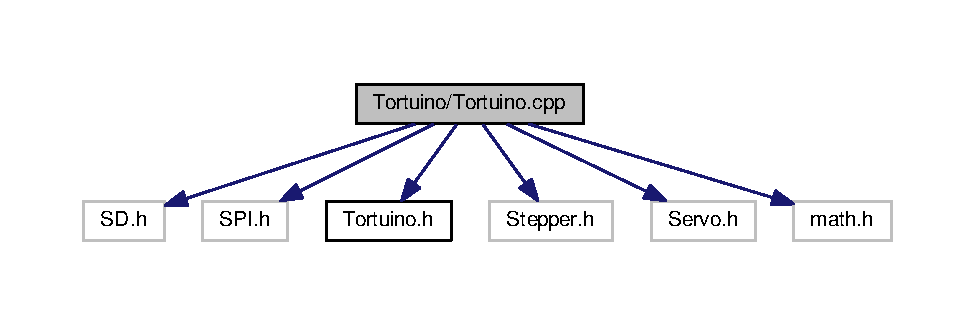
\includegraphics[width=350pt]{Tortuino_8cpp__incl}
\end{center}
\end{figure}
\subsection*{Fonctions}
\begin{DoxyCompactItemize}
\item 
int \hyperlink{Tortuino_8cpp_aafd65bcf38b0045f1e0ee681061a9e7c}{distance\+To\+Step} (float distance)
\begin{DoxyCompactList}\small\item\em Réalise la conversion d\textquotesingle{}une distance que le robot peut parcourir en un certain nombre de pas que chacun des deux moteurs pas à pas doit effectuer pour que le robot puisse avancer de la distance donnée. \end{DoxyCompactList}\item 
void \hyperlink{Tortuino_8cpp_a2af89837a61b0af5c06394e5956c81d0}{initialiser} ()
\begin{DoxyCompactList}\small\item\em Initialise la configuration du robot pour qu\textquotesingle{}il puisse correctement communiquer avec ses différents composants qui le constituent \+: le servomoteur, les moteurs pas à pas et le bouton de démarrage différé. \end{DoxyCompactList}\item 
void \hyperlink{Tortuino_8cpp_a48aa40d2f100ef290066c45fd4348553}{initialiser} (char couleur)
\begin{DoxyCompactList}\small\item\em Cette version de l\textquotesingle{}opération d\textquotesingle{}initialisation met en place une méthode pour calibrer chaque robot à souhait pour que les erreurs systématiques au moment de la rotation puissent être compensées. \end{DoxyCompactList}\item 
void \hyperlink{Tortuino_8cpp_ace2f9a05f9c51fcf5151c1e1c5ef107c}{initialiser} (float braquage)
\begin{DoxyCompactList}\small\item\em Cette version de l\textquotesingle{}opération d\textquotesingle{}initialisation est utile à la calibration d\textquotesingle{}un robot car affecte directement au rayon de braquage la moitié de la valeur fournie en entrée. \end{DoxyCompactList}\item 
void \hyperlink{Tortuino_8cpp_ac3d131be17dee64b89b0806bd4ee37b2}{attendre\+Bouton} ()
\begin{DoxyCompactList}\small\item\em Réalise l\textquotesingle{}attente nécessaire à la fonctionnalité du démarrage différé. \end{DoxyCompactList}\item 
void \hyperlink{Tortuino_8cpp_ad4869b51496adaf96ca447f5c7398197}{stopper} ()
\begin{DoxyCompactList}\small\item\em Permet de mettre à l\textquotesingle{}arrêt l\textquotesingle{}exécution en cours que réalise l\textquotesingle{}Arduino. \end{DoxyCompactList}\item 
void \hyperlink{Tortuino_8cpp_ab7928bf519ac707766463d32330ae02c}{vitesse} (int v)
\begin{DoxyCompactList}\small\item\em Règle la vitesse de rotation des moteurs pas à pas. \end{DoxyCompactList}\item 
void \hyperlink{Tortuino_8cpp_a64bb28327d74796c2c81845523b7425f}{avancer} (float distance)
\begin{DoxyCompactList}\small\item\em Fait avancer le robot Tortuino d\textquotesingle{}une distance donnée. \end{DoxyCompactList}\item 
void \hyperlink{Tortuino_8cpp_adb4b90c2b3dd8a5aba981068df36bba0}{reculer} (float distance)
\begin{DoxyCompactList}\small\item\em Fait reculer le robot Tortuino d\textquotesingle{}une distance donnée. \end{DoxyCompactList}\item 
void \hyperlink{Tortuino_8cpp_a68c284f58ca18c57a5937859031ec16b}{tourner\+Gauche} (float angle)
\begin{DoxyCompactList}\small\item\em Fait tourner sur place le robot Tortuino d\textquotesingle{}un angle fourni vers sa gauche. \end{DoxyCompactList}\item 
void \hyperlink{Tortuino_8cpp_aa9d442166cb63de9ad4e85e6540a276f}{tourner\+Droite} (float angle)
\begin{DoxyCompactList}\small\item\em Fait tourner sur place le robot Tortuino d\textquotesingle{}un angle fourni vers sa droite. \end{DoxyCompactList}\item 
void \hyperlink{Tortuino_8cpp_af6c422d84f31684d84208dd0a3828449}{monter\+Feutre} ()
\begin{DoxyCompactList}\small\item\em Place le feutre en position haute de telle manière qu\textquotesingle{}il ne touche pas la feuille en-\/dessous du robot, en supposant que le collier le tenant et permettant ce déplacement soit correctement ajusté. \end{DoxyCompactList}\item 
void \hyperlink{Tortuino_8cpp_a38b27067ab836a2120ab4946d4fccf63}{descendre\+Feutre} ()
\begin{DoxyCompactList}\small\item\em Place le feutre en position basse de telle manière qu\textquotesingle{}il touche la feuille en-\/dessous du robot, en supposant que le collier le tenant et permettant ce déplacement soit correctement ajusté. \end{DoxyCompactList}\end{DoxyCompactItemize}
\subsection*{Variables}
\begin{DoxyCompactItemize}
\item 
const int \hyperlink{Tortuino_8cpp_a0dffab4a0297ba1dfc85381688a235bb}{steps\+Per\+Revolution} = 64 $\ast$ 64 / 2
\begin{DoxyCompactList}\small\item\em Le nombre de pas par tour que réalise un moteur pas à pas ; c\textquotesingle{}est une donnée constructeur. \end{DoxyCompactList}\item 
float \hyperlink{Tortuino_8cpp_ac294c99f76085cbe8d1b91ae882532b6}{P\+E\+R\+I\+M\+E\+T\+ER} = M\+\_\+\+PI $\ast$ 9.\+2
\begin{DoxyCompactList}\small\item\em Le périmètre des roues du robot tel que mesuré avec le pneu. \end{DoxyCompactList}\item 
float \hyperlink{Tortuino_8cpp_a2090d1bfbb42f24c35995f26bce5d88d}{B\+R\+A\+Q\+U\+A\+GE} = 11.\+3 / 2
\begin{DoxyCompactList}\small\item\em Le rayon de braquage du robot. \end{DoxyCompactList}\item 
const int \hyperlink{Tortuino_8cpp_acb58d9f9a2f6fc5feee08a6b8608923b}{F\+E\+U\+T\+R\+E\+\_\+\+H\+A\+UT} = 50
\begin{DoxyCompactList}\small\item\em L\textquotesingle{}angle de la position haute du servomoteur. \end{DoxyCompactList}\item 
const int \hyperlink{Tortuino_8cpp_a2f3d019fd98fa45800ff50e070168428}{F\+E\+U\+T\+R\+E\+\_\+\+B\+AS} = 10
\begin{DoxyCompactList}\small\item\em L\textquotesingle{}angle de la position basse du servomoteur. \end{DoxyCompactList}\item 
const int \hyperlink{Tortuino_8cpp_a58fc84b520fc48bc331849155ce88f5d}{port\+Bouton} = 7
\begin{DoxyCompactList}\small\item\em Le numéro de la broche qui sert de port pour le bouton permettant le démarrage différé \+: 7. \end{DoxyCompactList}\item 
const int \hyperlink{Tortuino_8cpp_acb30e18355c39519e306b7aff1cf8d7e}{port\+Servo} = 9
\begin{DoxyCompactList}\small\item\em Le numéro de la broche pour le port du servomoteur \+: 9. \end{DoxyCompactList}\item 
const int \hyperlink{Tortuino_8cpp_a639b5a8ddf6d8835ceb24ef9ceb53795}{delai\+Bouton} = 10
\begin{DoxyCompactList}\small\item\em Le délai en ms entre chaque test du bouton. \end{DoxyCompactList}\item 
const int \hyperlink{Tortuino_8cpp_a0fbf55c6d4908a32d7594ce830c0da7e}{delai\+Monter\+Descendre} = 200
\begin{DoxyCompactList}\small\item\em Le délai en ms d\textquotesingle{}attente après l\textquotesingle{}envoi d\textquotesingle{}une commande au feutre. \end{DoxyCompactList}\item 
Stepper \hyperlink{Tortuino_8cpp_a42114b3d3de9e085781f2eecb975fe30}{stepper\+Left}
\begin{DoxyCompactList}\small\item\em L\textquotesingle{}objet qui sert à contrôler le moteur pas à pas de gauche et qui est relié aux ports 10 à 13. \end{DoxyCompactList}\item 
Stepper \hyperlink{Tortuino_8cpp_a9aacc3ab5a103b7b2287ea1569df491a}{stepper\+Right}
\begin{DoxyCompactList}\small\item\em L\textquotesingle{}objet qui sert à contrôler le moteur pas à pas de droite et qui est relié aux ports 2 à 5. \end{DoxyCompactList}\item 
Servo \hyperlink{Tortuino_8cpp_a79efceea669fb85a732c30f47cf7e59c}{servo}
\begin{DoxyCompactList}\small\item\em L\textquotesingle{}objet qui sert à contrôler le servomoteur soulevant et abaissant le feutre du robot. \end{DoxyCompactList}\end{DoxyCompactItemize}


\subsection{Description détaillée}
Ce fichier décrit les instructions de base pour contrôler le robot. 

\begin{DoxyAuthor}{Auteur}
Alexandre Comte 

Paul Mabileau \href{mailto:paulmabileau@hotmail.fr}{\tt paulmabileau@hotmail.\+fr} 

Florian Bescher 
\end{DoxyAuthor}
\begin{DoxyVersion}{Version}
1.\+2
\end{DoxyVersion}
Le fichier \hyperlink{Tortuino_8cpp}{Tortuino.\+cpp} rassemble les fonctionnalités essentielles au bon fonctionnement de la communication avec un robot Tortuino. Ces fonctionnalités sont principalement réalisées et mises à disposition au travers de fonctions qui les implémentent. Il y a aussi des paramètres en début de fichiers qui peuvent être modifiés à souhait pour adapter au mieux les programmes au robot qui sera manipulé au final \+: le calibrer. 

\subsection{Documentation des fonctions}
\mbox{\Hypertarget{Tortuino_8cpp_ac3d131be17dee64b89b0806bd4ee37b2}\label{Tortuino_8cpp_ac3d131be17dee64b89b0806bd4ee37b2}} 
\index{Tortuino.\+cpp@{Tortuino.\+cpp}!attendre\+Bouton@{attendre\+Bouton}}
\index{attendre\+Bouton@{attendre\+Bouton}!Tortuino.\+cpp@{Tortuino.\+cpp}}
\subsubsection{\texorpdfstring{attendre\+Bouton()}{attendreBouton()}}
{\footnotesize\ttfamily void attendre\+Bouton (\begin{DoxyParamCaption}{ }\end{DoxyParamCaption})}



Réalise l\textquotesingle{}attente nécessaire à la fonctionnalité du démarrage différé. 

L\textquotesingle{}exécution de cette fonction bloquera tant que le bouton en question n\textquotesingle{}a pas été appuyé. 

Définition à la ligne 127 du fichier Tortuino.\+cpp.

\mbox{\Hypertarget{Tortuino_8cpp_a64bb28327d74796c2c81845523b7425f}\label{Tortuino_8cpp_a64bb28327d74796c2c81845523b7425f}} 
\index{Tortuino.\+cpp@{Tortuino.\+cpp}!avancer@{avancer}}
\index{avancer@{avancer}!Tortuino.\+cpp@{Tortuino.\+cpp}}
\subsubsection{\texorpdfstring{avancer()}{avancer()}}
{\footnotesize\ttfamily void avancer (\begin{DoxyParamCaption}\item[{float}]{distance }\end{DoxyParamCaption})}



Fait avancer le robot Tortuino d\textquotesingle{}une distance donnée. 


\begin{DoxyParams}{Paramètres}
{\em distance} & La distance en centimètres à parcourir. \\
\hline
\end{DoxyParams}
\begin{DoxySeeAlso}{Voir également}
\hyperlink{Tortuino_8cpp_adb4b90c2b3dd8a5aba981068df36bba0}{reculer(float distance)} 
\end{DoxySeeAlso}


Définition à la ligne 167 du fichier Tortuino.\+cpp.

\mbox{\Hypertarget{Tortuino_8cpp_a38b27067ab836a2120ab4946d4fccf63}\label{Tortuino_8cpp_a38b27067ab836a2120ab4946d4fccf63}} 
\index{Tortuino.\+cpp@{Tortuino.\+cpp}!descendre\+Feutre@{descendre\+Feutre}}
\index{descendre\+Feutre@{descendre\+Feutre}!Tortuino.\+cpp@{Tortuino.\+cpp}}
\subsubsection{\texorpdfstring{descendre\+Feutre()}{descendreFeutre()}}
{\footnotesize\ttfamily void descendre\+Feutre (\begin{DoxyParamCaption}{ }\end{DoxyParamCaption})}



Place le feutre en position basse de telle manière qu\textquotesingle{}il touche la feuille en-\/dessous du robot, en supposant que le collier le tenant et permettant ce déplacement soit correctement ajusté. 

\begin{DoxySeeAlso}{Voir également}
\hyperlink{Tortuino_8cpp_af6c422d84f31684d84208dd0a3828449}{monter\+Feutre()} 
\end{DoxySeeAlso}


Définition à la ligne 243 du fichier Tortuino.\+cpp.

\mbox{\Hypertarget{Tortuino_8cpp_aafd65bcf38b0045f1e0ee681061a9e7c}\label{Tortuino_8cpp_aafd65bcf38b0045f1e0ee681061a9e7c}} 
\index{Tortuino.\+cpp@{Tortuino.\+cpp}!distance\+To\+Step@{distance\+To\+Step}}
\index{distance\+To\+Step@{distance\+To\+Step}!Tortuino.\+cpp@{Tortuino.\+cpp}}
\subsubsection{\texorpdfstring{distance\+To\+Step()}{distanceToStep()}}
{\footnotesize\ttfamily int distance\+To\+Step (\begin{DoxyParamCaption}\item[{float}]{distance }\end{DoxyParamCaption})}



Réalise la conversion d\textquotesingle{}une distance que le robot peut parcourir en un certain nombre de pas que chacun des deux moteurs pas à pas doit effectuer pour que le robot puisse avancer de la distance donnée. 

Cette conversion prend en compte les paramètres décrivant la géométrie du robot.


\begin{DoxyParams}{Paramètres}
{\em distance} & La distance linéaire en centimètres correspondant à un déplacement. \\
\hline
\end{DoxyParams}
\begin{DoxyReturn}{Renvoie}
Le nombre de pas permettant de réaliser le déplacement de la distance donnée. 
\end{DoxyReturn}


Définition à la ligne 55 du fichier Tortuino.\+cpp.

\mbox{\Hypertarget{Tortuino_8cpp_a2af89837a61b0af5c06394e5956c81d0}\label{Tortuino_8cpp_a2af89837a61b0af5c06394e5956c81d0}} 
\index{Tortuino.\+cpp@{Tortuino.\+cpp}!initialiser@{initialiser}}
\index{initialiser@{initialiser}!Tortuino.\+cpp@{Tortuino.\+cpp}}
\subsubsection{\texorpdfstring{initialiser()}{initialiser()}\hspace{0.1cm}{\footnotesize\ttfamily [1/3]}}
{\footnotesize\ttfamily void initialiser (\begin{DoxyParamCaption}{ }\end{DoxyParamCaption})}



Initialise la configuration du robot pour qu\textquotesingle{}il puisse correctement communiquer avec ses différents composants qui le constituent \+: le servomoteur, les moteurs pas à pas et le bouton de démarrage différé. 

Au cours de cette configuration, elle met le robot dans un état standard qui sera ainsi toujours le même au début de l\textquotesingle{}exécution de chaque essai \+: la vitesse de rotation des moteurs pas à pas est par défaut de 10 et le feutre est en position basse. Cette fonction à sa fin fait appel à \hyperlink{Tortuino_8cpp_ac3d131be17dee64b89b0806bd4ee37b2}{attendre\+Bouton()} qui bloquera tant que le bouton de démarrage différé n\textquotesingle{}est pas appuyé. 

Définition à la ligne 67 du fichier Tortuino.\+cpp.

\mbox{\Hypertarget{Tortuino_8cpp_a48aa40d2f100ef290066c45fd4348553}\label{Tortuino_8cpp_a48aa40d2f100ef290066c45fd4348553}} 
\index{Tortuino.\+cpp@{Tortuino.\+cpp}!initialiser@{initialiser}}
\index{initialiser@{initialiser}!Tortuino.\+cpp@{Tortuino.\+cpp}}
\subsubsection{\texorpdfstring{initialiser()}{initialiser()}\hspace{0.1cm}{\footnotesize\ttfamily [2/3]}}
{\footnotesize\ttfamily void initialiser (\begin{DoxyParamCaption}\item[{char}]{couleur }\end{DoxyParamCaption})}



Cette version de l\textquotesingle{}opération d\textquotesingle{}initialisation met en place une méthode pour calibrer chaque robot à souhait pour que les erreurs systématiques au moment de la rotation puissent être compensées. 

Le choix qui a été fait ici est de donner à chaque robot une couleur (par exemple de la plaquette d\textquotesingle{}expérimentation électrique) représentée par la première lettre de son écriture et qui l\textquotesingle{}identifie de manière unique. Ensuite, grâce à une correspondance établie au préalable, la valeur du rayon de braquage est affectée par cette fonction, retrouvant ainsi le calibrage effectué. ~\newline
 Le reste de l\textquotesingle{}initialisation est bien entendu aussi réalisé.


\begin{DoxyParams}{Paramètres}
{\em couleur} & La première lettre de la couleur identifiant le robot utilisé. \\
\hline
\end{DoxyParams}
\begin{DoxySeeAlso}{Voir également}
\hyperlink{Tortuino_8cpp_a2af89837a61b0af5c06394e5956c81d0}{initialiser()} 
\end{DoxySeeAlso}


Définition à la ligne 89 du fichier Tortuino.\+cpp.

\mbox{\Hypertarget{Tortuino_8cpp_ace2f9a05f9c51fcf5151c1e1c5ef107c}\label{Tortuino_8cpp_ace2f9a05f9c51fcf5151c1e1c5ef107c}} 
\index{Tortuino.\+cpp@{Tortuino.\+cpp}!initialiser@{initialiser}}
\index{initialiser@{initialiser}!Tortuino.\+cpp@{Tortuino.\+cpp}}
\subsubsection{\texorpdfstring{initialiser()}{initialiser()}\hspace{0.1cm}{\footnotesize\ttfamily [3/3]}}
{\footnotesize\ttfamily void initialiser (\begin{DoxyParamCaption}\item[{float}]{braquage }\end{DoxyParamCaption})}



Cette version de l\textquotesingle{}opération d\textquotesingle{}initialisation est utile à la calibration d\textquotesingle{}un robot car affecte directement au rayon de braquage la moitié de la valeur fournie en entrée. 

Le reste de l\textquotesingle{}initialisation est bien entendu aussi réalisé.


\begin{DoxyParams}{Paramètres}
{\em braquage} & La valeur du diamètre de braquage à utiliser. \\
\hline
\end{DoxyParams}


Définition à la ligne 118 du fichier Tortuino.\+cpp.

\mbox{\Hypertarget{Tortuino_8cpp_af6c422d84f31684d84208dd0a3828449}\label{Tortuino_8cpp_af6c422d84f31684d84208dd0a3828449}} 
\index{Tortuino.\+cpp@{Tortuino.\+cpp}!monter\+Feutre@{monter\+Feutre}}
\index{monter\+Feutre@{monter\+Feutre}!Tortuino.\+cpp@{Tortuino.\+cpp}}
\subsubsection{\texorpdfstring{monter\+Feutre()}{monterFeutre()}}
{\footnotesize\ttfamily void monter\+Feutre (\begin{DoxyParamCaption}{ }\end{DoxyParamCaption})}



Place le feutre en position haute de telle manière qu\textquotesingle{}il ne touche pas la feuille en-\/dessous du robot, en supposant que le collier le tenant et permettant ce déplacement soit correctement ajusté. 

\begin{DoxySeeAlso}{Voir également}
\hyperlink{Tortuino_8cpp_a38b27067ab836a2120ab4946d4fccf63}{descendre\+Feutre()} 
\end{DoxySeeAlso}


Définition à la ligne 231 du fichier Tortuino.\+cpp.

\mbox{\Hypertarget{Tortuino_8cpp_adb4b90c2b3dd8a5aba981068df36bba0}\label{Tortuino_8cpp_adb4b90c2b3dd8a5aba981068df36bba0}} 
\index{Tortuino.\+cpp@{Tortuino.\+cpp}!reculer@{reculer}}
\index{reculer@{reculer}!Tortuino.\+cpp@{Tortuino.\+cpp}}
\subsubsection{\texorpdfstring{reculer()}{reculer()}}
{\footnotesize\ttfamily void reculer (\begin{DoxyParamCaption}\item[{float}]{distance }\end{DoxyParamCaption})}



Fait reculer le robot Tortuino d\textquotesingle{}une distance donnée. 


\begin{DoxyParams}{Paramètres}
{\em distance} & La distance en centimètres à parcourir. \\
\hline
\end{DoxyParams}
\begin{DoxySeeAlso}{Voir également}
\hyperlink{Tortuino_8cpp_a64bb28327d74796c2c81845523b7425f}{avancer(float distance)} 
\end{DoxySeeAlso}


Définition à la ligne 185 du fichier Tortuino.\+cpp.

\mbox{\Hypertarget{Tortuino_8cpp_ad4869b51496adaf96ca447f5c7398197}\label{Tortuino_8cpp_ad4869b51496adaf96ca447f5c7398197}} 
\index{Tortuino.\+cpp@{Tortuino.\+cpp}!stopper@{stopper}}
\index{stopper@{stopper}!Tortuino.\+cpp@{Tortuino.\+cpp}}
\subsubsection{\texorpdfstring{stopper()}{stopper()}}
{\footnotesize\ttfamily void stopper (\begin{DoxyParamCaption}{ }\end{DoxyParamCaption})}



Permet de mettre à l\textquotesingle{}arrêt l\textquotesingle{}exécution en cours que réalise l\textquotesingle{}Arduino. 

Cette fonction peut se révéler utile si le croquis Arduino utilise la fonction loop() mais souhaite à un moment donné stopper le robot. 

Définition à la ligne 147 du fichier Tortuino.\+cpp.

\mbox{\Hypertarget{Tortuino_8cpp_aa9d442166cb63de9ad4e85e6540a276f}\label{Tortuino_8cpp_aa9d442166cb63de9ad4e85e6540a276f}} 
\index{Tortuino.\+cpp@{Tortuino.\+cpp}!tourner\+Droite@{tourner\+Droite}}
\index{tourner\+Droite@{tourner\+Droite}!Tortuino.\+cpp@{Tortuino.\+cpp}}
\subsubsection{\texorpdfstring{tourner\+Droite()}{tournerDroite()}}
{\footnotesize\ttfamily void tourner\+Droite (\begin{DoxyParamCaption}\item[{float}]{angle }\end{DoxyParamCaption})}



Fait tourner sur place le robot Tortuino d\textquotesingle{}un angle fourni vers sa droite. 

La rotation s\textquotesingle{}effectue autour de l\textquotesingle{}axe de décrit le feutre positionné dans l\textquotesingle{}emplacement prévu à cet effet, de sorte que s\textquotesingle{}il reste baisser lors de l\textquotesingle{}opération, cela ne laisse pas de cercle de tracé derrière le robot.


\begin{DoxyParams}{Paramètres}
{\em angle} & L\textquotesingle{}angle en degrés de rotation vers la gauche à effectuer. \\
\hline
\end{DoxyParams}
\begin{DoxySeeAlso}{Voir également}
\hyperlink{Tortuino_8cpp_a68c284f58ca18c57a5937859031ec16b}{tourner\+Gauche(float angle)} 
\end{DoxySeeAlso}


Définition à la ligne 220 du fichier Tortuino.\+cpp.

\mbox{\Hypertarget{Tortuino_8cpp_a68c284f58ca18c57a5937859031ec16b}\label{Tortuino_8cpp_a68c284f58ca18c57a5937859031ec16b}} 
\index{Tortuino.\+cpp@{Tortuino.\+cpp}!tourner\+Gauche@{tourner\+Gauche}}
\index{tourner\+Gauche@{tourner\+Gauche}!Tortuino.\+cpp@{Tortuino.\+cpp}}
\subsubsection{\texorpdfstring{tourner\+Gauche()}{tournerGauche()}}
{\footnotesize\ttfamily void tourner\+Gauche (\begin{DoxyParamCaption}\item[{float}]{angle }\end{DoxyParamCaption})}



Fait tourner sur place le robot Tortuino d\textquotesingle{}un angle fourni vers sa gauche. 

La rotation s\textquotesingle{}effectue autour de l\textquotesingle{}axe de décrit le feutre positionné dans l\textquotesingle{}emplacement prévu à cet effet, de sorte que s\textquotesingle{}il reste baisser lors de l\textquotesingle{}opération, cela ne laisse pas de cercle de tracé derrière le robot.


\begin{DoxyParams}{Paramètres}
{\em angle} & L\textquotesingle{}angle en degrés de rotation vers la gauche à effectuer. \\
\hline
\end{DoxyParams}
\begin{DoxySeeAlso}{Voir également}
\hyperlink{Tortuino_8cpp_aa9d442166cb63de9ad4e85e6540a276f}{tourner\+Droite(float angle)} 
\end{DoxySeeAlso}


Définition à la ligne 198 du fichier Tortuino.\+cpp.

\mbox{\Hypertarget{Tortuino_8cpp_ab7928bf519ac707766463d32330ae02c}\label{Tortuino_8cpp_ab7928bf519ac707766463d32330ae02c}} 
\index{Tortuino.\+cpp@{Tortuino.\+cpp}!vitesse@{vitesse}}
\index{vitesse@{vitesse}!Tortuino.\+cpp@{Tortuino.\+cpp}}
\subsubsection{\texorpdfstring{vitesse()}{vitesse()}}
{\footnotesize\ttfamily void vitesse (\begin{DoxyParamCaption}\item[{int}]{v }\end{DoxyParamCaption})}



Règle la vitesse de rotation des moteurs pas à pas. 


\begin{DoxyParams}{Paramètres}
{\em v} & La valeur entière de la vitesse à affecter aux moteurs pas à pas. \\
\hline
\end{DoxyParams}


Définition à la ligne 157 du fichier Tortuino.\+cpp.



\subsection{Documentation des variables}
\mbox{\Hypertarget{Tortuino_8cpp_a2090d1bfbb42f24c35995f26bce5d88d}\label{Tortuino_8cpp_a2090d1bfbb42f24c35995f26bce5d88d}} 
\index{Tortuino.\+cpp@{Tortuino.\+cpp}!B\+R\+A\+Q\+U\+A\+GE@{B\+R\+A\+Q\+U\+A\+GE}}
\index{B\+R\+A\+Q\+U\+A\+GE@{B\+R\+A\+Q\+U\+A\+GE}!Tortuino.\+cpp@{Tortuino.\+cpp}}
\subsubsection{\texorpdfstring{B\+R\+A\+Q\+U\+A\+GE}{BRAQUAGE}}
{\footnotesize\ttfamily float B\+R\+A\+Q\+U\+A\+GE = 11.\+3 / 2}



Le rayon de braquage du robot. 

C\textquotesingle{}est une valeur qui peut être amenée à être calibrée. 

Définition à la ligne 29 du fichier Tortuino.\+cpp.

\mbox{\Hypertarget{Tortuino_8cpp_a639b5a8ddf6d8835ceb24ef9ceb53795}\label{Tortuino_8cpp_a639b5a8ddf6d8835ceb24ef9ceb53795}} 
\index{Tortuino.\+cpp@{Tortuino.\+cpp}!delai\+Bouton@{delai\+Bouton}}
\index{delai\+Bouton@{delai\+Bouton}!Tortuino.\+cpp@{Tortuino.\+cpp}}
\subsubsection{\texorpdfstring{delai\+Bouton}{delaiBouton}}
{\footnotesize\ttfamily const int delai\+Bouton = 10}



Le délai en ms entre chaque test du bouton. 



Définition à la ligne 37 du fichier Tortuino.\+cpp.

\mbox{\Hypertarget{Tortuino_8cpp_a0fbf55c6d4908a32d7594ce830c0da7e}\label{Tortuino_8cpp_a0fbf55c6d4908a32d7594ce830c0da7e}} 
\index{Tortuino.\+cpp@{Tortuino.\+cpp}!delai\+Monter\+Descendre@{delai\+Monter\+Descendre}}
\index{delai\+Monter\+Descendre@{delai\+Monter\+Descendre}!Tortuino.\+cpp@{Tortuino.\+cpp}}
\subsubsection{\texorpdfstring{delai\+Monter\+Descendre}{delaiMonterDescendre}}
{\footnotesize\ttfamily const int delai\+Monter\+Descendre = 200}



Le délai en ms d\textquotesingle{}attente après l\textquotesingle{}envoi d\textquotesingle{}une commande au feutre. 

Paramétré empiriquement. 

Définition à la ligne 39 du fichier Tortuino.\+cpp.

\mbox{\Hypertarget{Tortuino_8cpp_a2f3d019fd98fa45800ff50e070168428}\label{Tortuino_8cpp_a2f3d019fd98fa45800ff50e070168428}} 
\index{Tortuino.\+cpp@{Tortuino.\+cpp}!F\+E\+U\+T\+R\+E\+\_\+\+B\+AS@{F\+E\+U\+T\+R\+E\+\_\+\+B\+AS}}
\index{F\+E\+U\+T\+R\+E\+\_\+\+B\+AS@{F\+E\+U\+T\+R\+E\+\_\+\+B\+AS}!Tortuino.\+cpp@{Tortuino.\+cpp}}
\subsubsection{\texorpdfstring{F\+E\+U\+T\+R\+E\+\_\+\+B\+AS}{FEUTRE\_BAS}}
{\footnotesize\ttfamily const int F\+E\+U\+T\+R\+E\+\_\+\+B\+AS = 10}



L\textquotesingle{}angle de la position basse du servomoteur. 

Il a été ajusté empiriquement. 

Définition à la ligne 32 du fichier Tortuino.\+cpp.

\mbox{\Hypertarget{Tortuino_8cpp_acb58d9f9a2f6fc5feee08a6b8608923b}\label{Tortuino_8cpp_acb58d9f9a2f6fc5feee08a6b8608923b}} 
\index{Tortuino.\+cpp@{Tortuino.\+cpp}!F\+E\+U\+T\+R\+E\+\_\+\+H\+A\+UT@{F\+E\+U\+T\+R\+E\+\_\+\+H\+A\+UT}}
\index{F\+E\+U\+T\+R\+E\+\_\+\+H\+A\+UT@{F\+E\+U\+T\+R\+E\+\_\+\+H\+A\+UT}!Tortuino.\+cpp@{Tortuino.\+cpp}}
\subsubsection{\texorpdfstring{F\+E\+U\+T\+R\+E\+\_\+\+H\+A\+UT}{FEUTRE\_HAUT}}
{\footnotesize\ttfamily const int F\+E\+U\+T\+R\+E\+\_\+\+H\+A\+UT = 50}



L\textquotesingle{}angle de la position haute du servomoteur. 

Il a été ajusté empiriquement. 

Définition à la ligne 31 du fichier Tortuino.\+cpp.

\mbox{\Hypertarget{Tortuino_8cpp_ac294c99f76085cbe8d1b91ae882532b6}\label{Tortuino_8cpp_ac294c99f76085cbe8d1b91ae882532b6}} 
\index{Tortuino.\+cpp@{Tortuino.\+cpp}!P\+E\+R\+I\+M\+E\+T\+ER@{P\+E\+R\+I\+M\+E\+T\+ER}}
\index{P\+E\+R\+I\+M\+E\+T\+ER@{P\+E\+R\+I\+M\+E\+T\+ER}!Tortuino.\+cpp@{Tortuino.\+cpp}}
\subsubsection{\texorpdfstring{P\+E\+R\+I\+M\+E\+T\+ER}{PERIMETER}}
{\footnotesize\ttfamily float P\+E\+R\+I\+M\+E\+T\+ER = M\+\_\+\+PI $\ast$ 9.\+2}



Le périmètre des roues du robot tel que mesuré avec le pneu. 



Définition à la ligne 28 du fichier Tortuino.\+cpp.

\mbox{\Hypertarget{Tortuino_8cpp_a58fc84b520fc48bc331849155ce88f5d}\label{Tortuino_8cpp_a58fc84b520fc48bc331849155ce88f5d}} 
\index{Tortuino.\+cpp@{Tortuino.\+cpp}!port\+Bouton@{port\+Bouton}}
\index{port\+Bouton@{port\+Bouton}!Tortuino.\+cpp@{Tortuino.\+cpp}}
\subsubsection{\texorpdfstring{port\+Bouton}{portBouton}}
{\footnotesize\ttfamily const int port\+Bouton = 7}



Le numéro de la broche qui sert de port pour le bouton permettant le démarrage différé \+: 7. 



Définition à la ligne 34 du fichier Tortuino.\+cpp.

\mbox{\Hypertarget{Tortuino_8cpp_acb30e18355c39519e306b7aff1cf8d7e}\label{Tortuino_8cpp_acb30e18355c39519e306b7aff1cf8d7e}} 
\index{Tortuino.\+cpp@{Tortuino.\+cpp}!port\+Servo@{port\+Servo}}
\index{port\+Servo@{port\+Servo}!Tortuino.\+cpp@{Tortuino.\+cpp}}
\subsubsection{\texorpdfstring{port\+Servo}{portServo}}
{\footnotesize\ttfamily const int port\+Servo = 9}



Le numéro de la broche pour le port du servomoteur \+: 9. 



Définition à la ligne 35 du fichier Tortuino.\+cpp.

\mbox{\Hypertarget{Tortuino_8cpp_a79efceea669fb85a732c30f47cf7e59c}\label{Tortuino_8cpp_a79efceea669fb85a732c30f47cf7e59c}} 
\index{Tortuino.\+cpp@{Tortuino.\+cpp}!servo@{servo}}
\index{servo@{servo}!Tortuino.\+cpp@{Tortuino.\+cpp}}
\subsubsection{\texorpdfstring{servo}{servo}}
{\footnotesize\ttfamily Servo servo}



L\textquotesingle{}objet qui sert à contrôler le servomoteur soulevant et abaissant le feutre du robot. 



Définition à la ligne 44 du fichier Tortuino.\+cpp.

\mbox{\Hypertarget{Tortuino_8cpp_a42114b3d3de9e085781f2eecb975fe30}\label{Tortuino_8cpp_a42114b3d3de9e085781f2eecb975fe30}} 
\index{Tortuino.\+cpp@{Tortuino.\+cpp}!stepper\+Left@{stepper\+Left}}
\index{stepper\+Left@{stepper\+Left}!Tortuino.\+cpp@{Tortuino.\+cpp}}
\subsubsection{\texorpdfstring{stepper\+Left}{stepperLeft}}
{\footnotesize\ttfamily Stepper stepper\+Left}



L\textquotesingle{}objet qui sert à contrôler le moteur pas à pas de gauche et qui est relié aux ports 10 à 13. 



Définition à la ligne 41 du fichier Tortuino.\+cpp.

\mbox{\Hypertarget{Tortuino_8cpp_a9aacc3ab5a103b7b2287ea1569df491a}\label{Tortuino_8cpp_a9aacc3ab5a103b7b2287ea1569df491a}} 
\index{Tortuino.\+cpp@{Tortuino.\+cpp}!stepper\+Right@{stepper\+Right}}
\index{stepper\+Right@{stepper\+Right}!Tortuino.\+cpp@{Tortuino.\+cpp}}
\subsubsection{\texorpdfstring{stepper\+Right}{stepperRight}}
{\footnotesize\ttfamily Stepper stepper\+Right}



L\textquotesingle{}objet qui sert à contrôler le moteur pas à pas de droite et qui est relié aux ports 2 à 5. 



Définition à la ligne 42 du fichier Tortuino.\+cpp.

\mbox{\Hypertarget{Tortuino_8cpp_a0dffab4a0297ba1dfc85381688a235bb}\label{Tortuino_8cpp_a0dffab4a0297ba1dfc85381688a235bb}} 
\index{Tortuino.\+cpp@{Tortuino.\+cpp}!steps\+Per\+Revolution@{steps\+Per\+Revolution}}
\index{steps\+Per\+Revolution@{steps\+Per\+Revolution}!Tortuino.\+cpp@{Tortuino.\+cpp}}
\subsubsection{\texorpdfstring{steps\+Per\+Revolution}{stepsPerRevolution}}
{\footnotesize\ttfamily const int steps\+Per\+Revolution = 64 $\ast$ 64 / 2}



Le nombre de pas par tour que réalise un moteur pas à pas ; c\textquotesingle{}est une donnée constructeur. 



Définition à la ligne 27 du fichier Tortuino.\+cpp.


\hypertarget{Tortuino_8h}{}\section{Référence du fichier Tortuino/\+Tortuino.h}
\label{Tortuino_8h}\index{Tortuino/\+Tortuino.\+h@{Tortuino/\+Tortuino.\+h}}


Définition des fonctions implémentées dans \hyperlink{Tortuino_8cpp}{Tortuino.\+cpp}.  


Ce graphe montre quels fichiers incluent directement ou indirectement ce fichier \+:\nopagebreak
\begin{figure}[H]
\begin{center}
\leavevmode
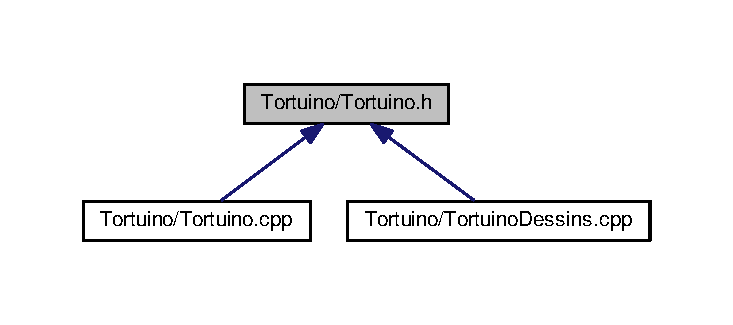
\includegraphics[width=350pt]{Tortuino_8h__dep__incl}
\end{center}
\end{figure}
\subsection*{Fonctions}
\begin{DoxyCompactItemize}
\item 
void \hyperlink{Tortuino_8h_a2af89837a61b0af5c06394e5956c81d0}{initialiser} ()
\begin{DoxyCompactList}\small\item\em Initialise la configuration du robot pour qu\textquotesingle{}il puisse correctement communiquer avec ses différents composants qui le constituent \+: le servomoteur, les moteurs pas à pas et le bouton de démarrage différé. \end{DoxyCompactList}\item 
void \hyperlink{Tortuino_8h_ace2f9a05f9c51fcf5151c1e1c5ef107c}{initialiser} (float braquage)
\begin{DoxyCompactList}\small\item\em Cette version de l\textquotesingle{}opération d\textquotesingle{}initialisation est utile à la calibration d\textquotesingle{}un robot car affecte directement au rayon de braquage la valeur fournie en entrée. \end{DoxyCompactList}\item 
void \hyperlink{Tortuino_8h_a48aa40d2f100ef290066c45fd4348553}{initialiser} (char couleur)
\begin{DoxyCompactList}\small\item\em Cette version de l\textquotesingle{}opération d\textquotesingle{}initialisation met en place une méthode pour calibrer chaque robot à souhait pour que les erreurs systématiques au moment de la rotation puissent être compensées. \end{DoxyCompactList}\item 
void \hyperlink{Tortuino_8h_ac3d131be17dee64b89b0806bd4ee37b2}{attendre\+Bouton} ()
\begin{DoxyCompactList}\small\item\em Réalise l\textquotesingle{}attente nécessaire à la fonctionnalité du démarrage différé. \end{DoxyCompactList}\item 
void \hyperlink{Tortuino_8h_ad4869b51496adaf96ca447f5c7398197}{stopper} ()
\begin{DoxyCompactList}\small\item\em Permet de mettre à l\textquotesingle{}arrêt l\textquotesingle{}exécution en cours que réalise l\textquotesingle{}Arduino. \end{DoxyCompactList}\item 
void \hyperlink{Tortuino_8h_ab7928bf519ac707766463d32330ae02c}{vitesse} (int v)
\begin{DoxyCompactList}\small\item\em Règle la vitesse de rotation des moteurs pas à pas. \end{DoxyCompactList}\item 
void \hyperlink{Tortuino_8h_a64bb28327d74796c2c81845523b7425f}{avancer} (float distance)
\begin{DoxyCompactList}\small\item\em Fait avancer le robot Tortuino d\textquotesingle{}une distance donnée. \end{DoxyCompactList}\item 
void \hyperlink{Tortuino_8h_adb4b90c2b3dd8a5aba981068df36bba0}{reculer} (float distance)
\begin{DoxyCompactList}\small\item\em Fait reculer le robot Tortuino d\textquotesingle{}une distance donnée. \end{DoxyCompactList}\item 
void \hyperlink{Tortuino_8h_a68c284f58ca18c57a5937859031ec16b}{tourner\+Gauche} (float angle)
\begin{DoxyCompactList}\small\item\em Fait tourner sur place le robot Tortuino d\textquotesingle{}un angle fourni vers sa gauche. \end{DoxyCompactList}\item 
void \hyperlink{Tortuino_8h_aa9d442166cb63de9ad4e85e6540a276f}{tourner\+Droite} (float angle)
\begin{DoxyCompactList}\small\item\em Fait tourner sur place le robot Tortuino d\textquotesingle{}un angle fourni vers sa droite. \end{DoxyCompactList}\item 
void \hyperlink{Tortuino_8h_af6c422d84f31684d84208dd0a3828449}{monter\+Feutre} ()
\begin{DoxyCompactList}\small\item\em Place le feutre en position haute de telle manière qu\textquotesingle{}il ne touche pas la feuille en-\/dessous du robot, en supposant que le collier le tenant et permettant ce déplacement soit correctement ajusté. \end{DoxyCompactList}\item 
void \hyperlink{Tortuino_8h_a38b27067ab836a2120ab4946d4fccf63}{descendre\+Feutre} ()
\begin{DoxyCompactList}\small\item\em Place le feutre en position basse de telle manière qu\textquotesingle{}il touche la feuille en-\/dessous du robot, en supposant que le collier le tenant et permettant ce déplacement soit correctement ajusté. \end{DoxyCompactList}\end{DoxyCompactItemize}


\subsection{Description détaillée}
Définition des fonctions implémentées dans \hyperlink{Tortuino_8cpp}{Tortuino.\+cpp}. 

\begin{DoxyVersion}{Version}
1.\+1 
\end{DoxyVersion}
\begin{DoxyAuthor}{Auteur}
Paul Mabileau \href{mailto:paulmabileau@hotmail.fr}{\tt paulmabileau@hotmail.\+fr}
\end{DoxyAuthor}
Ce fichier constitue l\textquotesingle{}en-\/tête de \hyperlink{Tortuino_8cpp}{Tortuino.\+cpp}. Il permet de préciser ce qui sera rendu accessible à d\textquotesingle{}autres programmes. Ici, ce sont des fonctions. 

\subsection{Documentation des fonctions}
\mbox{\Hypertarget{Tortuino_8h_ac3d131be17dee64b89b0806bd4ee37b2}\label{Tortuino_8h_ac3d131be17dee64b89b0806bd4ee37b2}} 
\index{Tortuino.\+h@{Tortuino.\+h}!attendre\+Bouton@{attendre\+Bouton}}
\index{attendre\+Bouton@{attendre\+Bouton}!Tortuino.\+h@{Tortuino.\+h}}
\subsubsection{\texorpdfstring{attendre\+Bouton()}{attendreBouton()}}
{\footnotesize\ttfamily void attendre\+Bouton (\begin{DoxyParamCaption}{ }\end{DoxyParamCaption})}



Réalise l\textquotesingle{}attente nécessaire à la fonctionnalité du démarrage différé. 

L\textquotesingle{}exécution de cette fonction bloquera tant que le bouton en question n\textquotesingle{}a pas été appuyé. 

Définition à la ligne 127 du fichier Tortuino.\+cpp.

\mbox{\Hypertarget{Tortuino_8h_a64bb28327d74796c2c81845523b7425f}\label{Tortuino_8h_a64bb28327d74796c2c81845523b7425f}} 
\index{Tortuino.\+h@{Tortuino.\+h}!avancer@{avancer}}
\index{avancer@{avancer}!Tortuino.\+h@{Tortuino.\+h}}
\subsubsection{\texorpdfstring{avancer()}{avancer()}}
{\footnotesize\ttfamily void avancer (\begin{DoxyParamCaption}\item[{float}]{distance }\end{DoxyParamCaption})}



Fait avancer le robot Tortuino d\textquotesingle{}une distance donnée. 


\begin{DoxyParams}{Paramètres}
{\em distance} & La distance en centimètres à parcourir. \\
\hline
\end{DoxyParams}
\begin{DoxySeeAlso}{Voir également}
\hyperlink{Tortuino_8cpp_adb4b90c2b3dd8a5aba981068df36bba0}{reculer(float distance)} 
\end{DoxySeeAlso}


Définition à la ligne 167 du fichier Tortuino.\+cpp.

\mbox{\Hypertarget{Tortuino_8h_a38b27067ab836a2120ab4946d4fccf63}\label{Tortuino_8h_a38b27067ab836a2120ab4946d4fccf63}} 
\index{Tortuino.\+h@{Tortuino.\+h}!descendre\+Feutre@{descendre\+Feutre}}
\index{descendre\+Feutre@{descendre\+Feutre}!Tortuino.\+h@{Tortuino.\+h}}
\subsubsection{\texorpdfstring{descendre\+Feutre()}{descendreFeutre()}}
{\footnotesize\ttfamily void descendre\+Feutre (\begin{DoxyParamCaption}{ }\end{DoxyParamCaption})}



Place le feutre en position basse de telle manière qu\textquotesingle{}il touche la feuille en-\/dessous du robot, en supposant que le collier le tenant et permettant ce déplacement soit correctement ajusté. 

\begin{DoxySeeAlso}{Voir également}
\hyperlink{Tortuino_8cpp_af6c422d84f31684d84208dd0a3828449}{monter\+Feutre()} 
\end{DoxySeeAlso}


Définition à la ligne 243 du fichier Tortuino.\+cpp.

\mbox{\Hypertarget{Tortuino_8h_a2af89837a61b0af5c06394e5956c81d0}\label{Tortuino_8h_a2af89837a61b0af5c06394e5956c81d0}} 
\index{Tortuino.\+h@{Tortuino.\+h}!initialiser@{initialiser}}
\index{initialiser@{initialiser}!Tortuino.\+h@{Tortuino.\+h}}
\subsubsection{\texorpdfstring{initialiser()}{initialiser()}\hspace{0.1cm}{\footnotesize\ttfamily [1/3]}}
{\footnotesize\ttfamily void initialiser (\begin{DoxyParamCaption}{ }\end{DoxyParamCaption})}



Initialise la configuration du robot pour qu\textquotesingle{}il puisse correctement communiquer avec ses différents composants qui le constituent \+: le servomoteur, les moteurs pas à pas et le bouton de démarrage différé. 

Au cours de cette configuration, elle met le robot dans un état standard qui sera ainsi toujours le même au début de l\textquotesingle{}exécution de chaque essai \+: la vitesse de rotation des moteurs pas à pas est par défaut de 10 et le feutre est en position basse. Cette fonction à sa fin fait appel à \hyperlink{Tortuino_8cpp_ac3d131be17dee64b89b0806bd4ee37b2}{attendre\+Bouton()} qui bloquera tant que le bouton de démarrage différé n\textquotesingle{}est pas appuyé. 

Définition à la ligne 67 du fichier Tortuino.\+cpp.

\mbox{\Hypertarget{Tortuino_8h_ace2f9a05f9c51fcf5151c1e1c5ef107c}\label{Tortuino_8h_ace2f9a05f9c51fcf5151c1e1c5ef107c}} 
\index{Tortuino.\+h@{Tortuino.\+h}!initialiser@{initialiser}}
\index{initialiser@{initialiser}!Tortuino.\+h@{Tortuino.\+h}}
\subsubsection{\texorpdfstring{initialiser()}{initialiser()}\hspace{0.1cm}{\footnotesize\ttfamily [2/3]}}
{\footnotesize\ttfamily void initialiser (\begin{DoxyParamCaption}\item[{float}]{braquage }\end{DoxyParamCaption})}



Cette version de l\textquotesingle{}opération d\textquotesingle{}initialisation est utile à la calibration d\textquotesingle{}un robot car affecte directement au rayon de braquage la valeur fournie en entrée. 

Le reste de l\textquotesingle{}initialisation est bien entendu aussi réalisé.


\begin{DoxyParams}{Paramètres}
{\em braquage} & La valeur du rayon de braquage à utiliser. \\
\hline
\end{DoxyParams}


Définition à la ligne 118 du fichier Tortuino.\+cpp.

\mbox{\Hypertarget{Tortuino_8h_a48aa40d2f100ef290066c45fd4348553}\label{Tortuino_8h_a48aa40d2f100ef290066c45fd4348553}} 
\index{Tortuino.\+h@{Tortuino.\+h}!initialiser@{initialiser}}
\index{initialiser@{initialiser}!Tortuino.\+h@{Tortuino.\+h}}
\subsubsection{\texorpdfstring{initialiser()}{initialiser()}\hspace{0.1cm}{\footnotesize\ttfamily [3/3]}}
{\footnotesize\ttfamily void initialiser (\begin{DoxyParamCaption}\item[{char}]{couleur }\end{DoxyParamCaption})}



Cette version de l\textquotesingle{}opération d\textquotesingle{}initialisation met en place une méthode pour calibrer chaque robot à souhait pour que les erreurs systématiques au moment de la rotation puissent être compensées. 

Le choix qui a été fait ici est de donner à chaque robot une couleur (par exemple de la plaquette d\textquotesingle{}expérimentation électrique) représentée par la première lettre de son écriture et qui l\textquotesingle{}identifie de manière unique. Ensuite, grâce à une correspondance établie au préalable, la valeur du rayon de braquage est affectée par cette fonction, retrouvant ainsi le calibrage effectué. ~\newline
 Le reste de l\textquotesingle{}initialisation est bien entendu aussi réalisé.


\begin{DoxyParams}{Paramètres}
{\em couleur} & La première lettre de la couleur identifiant le robot utilisé. \\
\hline
\end{DoxyParams}
\begin{DoxySeeAlso}{Voir également}
\hyperlink{Tortuino_8cpp_a2af89837a61b0af5c06394e5956c81d0}{initialiser()} 
\end{DoxySeeAlso}


Définition à la ligne 89 du fichier Tortuino.\+cpp.

\mbox{\Hypertarget{Tortuino_8h_af6c422d84f31684d84208dd0a3828449}\label{Tortuino_8h_af6c422d84f31684d84208dd0a3828449}} 
\index{Tortuino.\+h@{Tortuino.\+h}!monter\+Feutre@{monter\+Feutre}}
\index{monter\+Feutre@{monter\+Feutre}!Tortuino.\+h@{Tortuino.\+h}}
\subsubsection{\texorpdfstring{monter\+Feutre()}{monterFeutre()}}
{\footnotesize\ttfamily void monter\+Feutre (\begin{DoxyParamCaption}{ }\end{DoxyParamCaption})}



Place le feutre en position haute de telle manière qu\textquotesingle{}il ne touche pas la feuille en-\/dessous du robot, en supposant que le collier le tenant et permettant ce déplacement soit correctement ajusté. 

\begin{DoxySeeAlso}{Voir également}
\hyperlink{Tortuino_8cpp_a38b27067ab836a2120ab4946d4fccf63}{descendre\+Feutre()} 
\end{DoxySeeAlso}


Définition à la ligne 231 du fichier Tortuino.\+cpp.

\mbox{\Hypertarget{Tortuino_8h_adb4b90c2b3dd8a5aba981068df36bba0}\label{Tortuino_8h_adb4b90c2b3dd8a5aba981068df36bba0}} 
\index{Tortuino.\+h@{Tortuino.\+h}!reculer@{reculer}}
\index{reculer@{reculer}!Tortuino.\+h@{Tortuino.\+h}}
\subsubsection{\texorpdfstring{reculer()}{reculer()}}
{\footnotesize\ttfamily void reculer (\begin{DoxyParamCaption}\item[{float}]{distance }\end{DoxyParamCaption})}



Fait reculer le robot Tortuino d\textquotesingle{}une distance donnée. 


\begin{DoxyParams}{Paramètres}
{\em distance} & La distance en centimètres à parcourir. \\
\hline
\end{DoxyParams}
\begin{DoxySeeAlso}{Voir également}
\hyperlink{Tortuino_8cpp_a64bb28327d74796c2c81845523b7425f}{avancer(float distance)} 
\end{DoxySeeAlso}


Définition à la ligne 185 du fichier Tortuino.\+cpp.

\mbox{\Hypertarget{Tortuino_8h_ad4869b51496adaf96ca447f5c7398197}\label{Tortuino_8h_ad4869b51496adaf96ca447f5c7398197}} 
\index{Tortuino.\+h@{Tortuino.\+h}!stopper@{stopper}}
\index{stopper@{stopper}!Tortuino.\+h@{Tortuino.\+h}}
\subsubsection{\texorpdfstring{stopper()}{stopper()}}
{\footnotesize\ttfamily void stopper (\begin{DoxyParamCaption}{ }\end{DoxyParamCaption})}



Permet de mettre à l\textquotesingle{}arrêt l\textquotesingle{}exécution en cours que réalise l\textquotesingle{}Arduino. 

Cette fonction peut se révéler utile si le croquis Arduino utilise la fonction loop() mais souhaite à un moment donné stopper le robot. 

Définition à la ligne 147 du fichier Tortuino.\+cpp.

\mbox{\Hypertarget{Tortuino_8h_aa9d442166cb63de9ad4e85e6540a276f}\label{Tortuino_8h_aa9d442166cb63de9ad4e85e6540a276f}} 
\index{Tortuino.\+h@{Tortuino.\+h}!tourner\+Droite@{tourner\+Droite}}
\index{tourner\+Droite@{tourner\+Droite}!Tortuino.\+h@{Tortuino.\+h}}
\subsubsection{\texorpdfstring{tourner\+Droite()}{tournerDroite()}}
{\footnotesize\ttfamily void tourner\+Droite (\begin{DoxyParamCaption}\item[{float}]{angle }\end{DoxyParamCaption})}



Fait tourner sur place le robot Tortuino d\textquotesingle{}un angle fourni vers sa droite. 

La rotation s\textquotesingle{}effectue autour de l\textquotesingle{}axe de décrit le feutre positionné dans l\textquotesingle{}emplacement prévu à cet effet, de sorte que s\textquotesingle{}il reste baisser lors de l\textquotesingle{}opération, cela ne laisse pas de cercle de tracé derrière le robot.


\begin{DoxyParams}{Paramètres}
{\em angle} & L\textquotesingle{}angle en degrés de rotation vers la gauche à effectuer. \\
\hline
\end{DoxyParams}
\begin{DoxySeeAlso}{Voir également}
\hyperlink{Tortuino_8cpp_a68c284f58ca18c57a5937859031ec16b}{tourner\+Gauche(float angle)} 
\end{DoxySeeAlso}


Définition à la ligne 220 du fichier Tortuino.\+cpp.

\mbox{\Hypertarget{Tortuino_8h_a68c284f58ca18c57a5937859031ec16b}\label{Tortuino_8h_a68c284f58ca18c57a5937859031ec16b}} 
\index{Tortuino.\+h@{Tortuino.\+h}!tourner\+Gauche@{tourner\+Gauche}}
\index{tourner\+Gauche@{tourner\+Gauche}!Tortuino.\+h@{Tortuino.\+h}}
\subsubsection{\texorpdfstring{tourner\+Gauche()}{tournerGauche()}}
{\footnotesize\ttfamily void tourner\+Gauche (\begin{DoxyParamCaption}\item[{float}]{angle }\end{DoxyParamCaption})}



Fait tourner sur place le robot Tortuino d\textquotesingle{}un angle fourni vers sa gauche. 

La rotation s\textquotesingle{}effectue autour de l\textquotesingle{}axe de décrit le feutre positionné dans l\textquotesingle{}emplacement prévu à cet effet, de sorte que s\textquotesingle{}il reste baisser lors de l\textquotesingle{}opération, cela ne laisse pas de cercle de tracé derrière le robot.


\begin{DoxyParams}{Paramètres}
{\em angle} & L\textquotesingle{}angle en degrés de rotation vers la gauche à effectuer. \\
\hline
\end{DoxyParams}
\begin{DoxySeeAlso}{Voir également}
\hyperlink{Tortuino_8cpp_aa9d442166cb63de9ad4e85e6540a276f}{tourner\+Droite(float angle)} 
\end{DoxySeeAlso}


Définition à la ligne 198 du fichier Tortuino.\+cpp.

\mbox{\Hypertarget{Tortuino_8h_ab7928bf519ac707766463d32330ae02c}\label{Tortuino_8h_ab7928bf519ac707766463d32330ae02c}} 
\index{Tortuino.\+h@{Tortuino.\+h}!vitesse@{vitesse}}
\index{vitesse@{vitesse}!Tortuino.\+h@{Tortuino.\+h}}
\subsubsection{\texorpdfstring{vitesse()}{vitesse()}}
{\footnotesize\ttfamily void vitesse (\begin{DoxyParamCaption}\item[{int}]{v }\end{DoxyParamCaption})}



Règle la vitesse de rotation des moteurs pas à pas. 


\begin{DoxyParams}{Paramètres}
{\em v} & La valeur entière de la vitesse à affecter aux moteurs pas à pas. \\
\hline
\end{DoxyParams}


Définition à la ligne 157 du fichier Tortuino.\+cpp.


\hypertarget{TortuinoDessins_8cpp}{}\section{Référence du fichier Tortuino/\+Tortuino\+Dessins.cpp}
\label{TortuinoDessins_8cpp}\index{Tortuino/\+Tortuino\+Dessins.\+cpp@{Tortuino/\+Tortuino\+Dessins.\+cpp}}


Ce fichier met à disposition quelques dessins qui peuvent être intéressants d\textquotesingle{}essayer.  


{\ttfamily \#include \char`\"{}Tortuino.\+h\char`\"{}}\newline
{\ttfamily \#include \char`\"{}Tortuino\+Dessins.\+h\char`\"{}}\newline
{\ttfamily \#include $<$math.\+h$>$}\newline
Graphe des dépendances par inclusion de Tortuino\+Dessins.\+cpp\+:\nopagebreak
\begin{figure}[H]
\begin{center}
\leavevmode
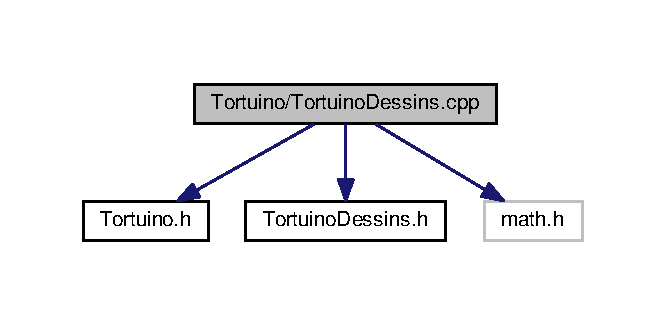
\includegraphics[width=320pt]{TortuinoDessins_8cpp__incl}
\end{center}
\end{figure}
\subsection*{Fonctions}
\begin{DoxyCompactItemize}
\item 
void \hyperlink{TortuinoDessins_8cpp_ada93849cc1680d0d43bf6f9c1de954b2}{polygone\+Regulier} (int nb\+Cotes, float taille\+Cote)
\begin{DoxyCompactList}\small\item\em Fait tracer au robot un polygone régulier en fonction du nombre de côtés souhaités et de la taille de chacun de ces côtés. \end{DoxyCompactList}\item 
void \hyperlink{TortuinoDessins_8cpp_afa3484b3831c738502a4c381600397ea}{triangle} (float taille\+Cote)
\begin{DoxyCompactList}\small\item\em Trace un triangle equilatéral d\textquotesingle{}une certaine taille. \end{DoxyCompactList}\item 
void \hyperlink{TortuinoDessins_8cpp_a8fd6d1d3aad9c0c10525e5c8244a6ce1}{carre} (float taille\+Cote)
\begin{DoxyCompactList}\small\item\em Trace un carré d\textquotesingle{}une certaine taille. \end{DoxyCompactList}\item 
void \hyperlink{TortuinoDessins_8cpp_a57189e3fe807009b1595778589a16be9}{cercle} (float rayon)
\begin{DoxyCompactList}\small\item\em Cette fonction est une tentative de réalisation d\textquotesingle{}un cercle automatiquement avec juste le rayon souhaité en entrée. \end{DoxyCompactList}\item 
void \hyperlink{TortuinoDessins_8cpp_a39c1c8ca3b979edec7d841f1a71e50f1}{arbre} (int nb\+Niveaux, float taille\+Tronc)
\begin{DoxyCompactList}\small\item\em Trace un arbre récursivement dont l\textquotesingle{}angle entre les branches est de 90 degrés et qui est symétrique par rapport à l\textquotesingle{}axe formé par son tronc. \end{DoxyCompactList}\item 
void \hyperlink{TortuinoDessins_8cpp_ac8968b78a962de5017b660c5e8e37513}{arbre\+Symetrique} (int nb\+Niveaux, float taille\+Tronc, float angle\+Separation)
\begin{DoxyCompactList}\small\item\em Trace un arbre récursivement dont l\textquotesingle{}angle entre les branches peut être précisé et qui est symétrique par rapport à l\textquotesingle{}axe formé par son tronc. \end{DoxyCompactList}\item 
void \hyperlink{TortuinoDessins_8cpp_a29fa4a540a63b4e05fe0aee6d5b522c0}{arbre\+Asymetrique} (int nb\+Niveaux, float taille\+Tronc, float angle\+Separation, float angle\+Inclinaison)
\begin{DoxyCompactList}\small\item\em Trace un arbre récursivement dont l\textquotesingle{}angle entre les branches et l\textquotesingle{}angle entre la branche de gauche et la branche mère moins 45 degrés peuvent être précisés \+: il est asymétrique par rapport à l\textquotesingle{}axe formé par son tronc. \end{DoxyCompactList}\item 
void \hyperlink{TortuinoDessins_8cpp_a170bac7a60b14659e63b81c8eefac3dd}{sapin} (int nb\+Niveaux, float taille\+Tronc)
\begin{DoxyCompactList}\small\item\em Utilise deux arbres asymétriques pour tracer un sapin, c\textquotesingle{}est-\/à-\/dire un arbre où chaque branche se sépare en trois autres \+: une continuant vers le haut (le tronc donc) et deux horizontales sur le côté (les branches donc). \end{DoxyCompactList}\item 
void \hyperlink{TortuinoDessins_8cpp_af86cf0f8acc522368a052c765047a3a1}{courbe\+Von\+Koch} (int nb\+Niveaux, float taille)
\begin{DoxyCompactList}\small\item\em Trace une \href{https://fr.wikipedia.org/wiki/Flocon_de_Koch#Courbe_de_Koch}{\tt courbe de Von Koch} paramétrée par son niveau et la taille du segment de départ. \end{DoxyCompactList}\item 
void \hyperlink{TortuinoDessins_8cpp_afa05db28401a10aa6c4625a2de482484}{flocon} (int nb\+Niveaux, float taille)
\begin{DoxyCompactList}\small\item\em Trace un \href{https://fr.wikipedia.org/wiki/Flocon_de_Koch#Flocon_de_Koch}{\tt flocon de Von Koch} paramétré par son niveau et la taille du segment de départ. \end{DoxyCompactList}\item 
void \hyperlink{TortuinoDessins_8cpp_a0c851f0f43370a65c2da38436be9a764}{triangle\+Sierpinski} (int nb\+Niveaux, float taille)
\begin{DoxyCompactList}\small\item\em Trace un \href{https://fr.wikipedia.org/wiki/Triangle_de_Sierpi%C5%84ski}{\tt triangle de Sierpiński} paramétré par son niveau et la taille globale du triangle. \end{DoxyCompactList}\end{DoxyCompactItemize}


\subsection{Description détaillée}
Ce fichier met à disposition quelques dessins qui peuvent être intéressants d\textquotesingle{}essayer. 

\begin{DoxyAuthor}{Auteur}
Paul Mabileau \href{mailto:paulmabileau@hotmail.fr}{\tt paulmabileau@hotmail.\+fr} 
\end{DoxyAuthor}
\begin{DoxyVersion}{Version}
1.\+2
\end{DoxyVersion}
Le fichier \hyperlink{TortuinoDessins_8cpp}{Tortuino\+Dessins.\+cpp} implémente un ensemble de fonctions réalisant quelques dessins plus ou moins complexes. Les dessins les plus simples sont par exemple des polygones réguliers tels qu\textquotesingle{}un triangle, un carré, un hexagone, ... les plus compliqués utilise des motifs récursifs, ce qui est moins simple à programmer, mais tout à fait agréable à contempler, comme par exemple un arbre avec différentes variantes, un flocon ou encore le triangle de Sierpiński. 

\subsection{Documentation des fonctions}
\mbox{\Hypertarget{TortuinoDessins_8cpp_a39c1c8ca3b979edec7d841f1a71e50f1}\label{TortuinoDessins_8cpp_a39c1c8ca3b979edec7d841f1a71e50f1}} 
\index{Tortuino\+Dessins.\+cpp@{Tortuino\+Dessins.\+cpp}!arbre@{arbre}}
\index{arbre@{arbre}!Tortuino\+Dessins.\+cpp@{Tortuino\+Dessins.\+cpp}}
\subsubsection{\texorpdfstring{arbre()}{arbre()}}
{\footnotesize\ttfamily void arbre (\begin{DoxyParamCaption}\item[{int}]{nb\+Niveaux,  }\item[{float}]{taille\+Tronc }\end{DoxyParamCaption})}



Trace un arbre récursivement dont l\textquotesingle{}angle entre les branches est de 90 degrés et qui est symétrique par rapport à l\textquotesingle{}axe formé par son tronc. 

C\textquotesingle{}est donc un cas particulier de \hyperlink{TortuinoDessins_8cpp_ac8968b78a962de5017b660c5e8e37513}{arbre\+Symetrique(int nb\+Niveaux, float taille\+Tronc, float angle\+Separation)}.


\begin{DoxyParams}{Paramètres}
{\em nb\+Niveaux} & Le nombre de niveaux que l\textquotesingle{}arbre comprendra, c\textquotesingle{}est-\/à-\/dire le nombre de fois moins un que l\textquotesingle{}arbre va se séparer ou autrement dit la distance en nombre de branches entre la racine et chaque feuille. \\
\hline
{\em taille\+Tronc} & La taille du tronc de départ. Les branches qui en partiront auront leurs tailles d\textquotesingle{}un tier plus petites. \\
\hline
\end{DoxyParams}


Définition à la ligne 86 du fichier Tortuino\+Dessins.\+cpp.

\mbox{\Hypertarget{TortuinoDessins_8cpp_a29fa4a540a63b4e05fe0aee6d5b522c0}\label{TortuinoDessins_8cpp_a29fa4a540a63b4e05fe0aee6d5b522c0}} 
\index{Tortuino\+Dessins.\+cpp@{Tortuino\+Dessins.\+cpp}!arbre\+Asymetrique@{arbre\+Asymetrique}}
\index{arbre\+Asymetrique@{arbre\+Asymetrique}!Tortuino\+Dessins.\+cpp@{Tortuino\+Dessins.\+cpp}}
\subsubsection{\texorpdfstring{arbre\+Asymetrique()}{arbreAsymetrique()}}
{\footnotesize\ttfamily void arbre\+Asymetrique (\begin{DoxyParamCaption}\item[{int}]{nb\+Niveaux,  }\item[{float}]{taille\+Tronc,  }\item[{float}]{angle\+Separation,  }\item[{float}]{angle\+Inclinaison }\end{DoxyParamCaption})}



Trace un arbre récursivement dont l\textquotesingle{}angle entre les branches et l\textquotesingle{}angle entre la branche de gauche et la branche mère moins 45 degrés peuvent être précisés \+: il est asymétrique par rapport à l\textquotesingle{}axe formé par son tronc. 

Il généralise donc un arbre.


\begin{DoxyParams}{Paramètres}
{\em nb\+Niveaux} & Le nombre de niveaux que l\textquotesingle{}arbre comprendra, c\textquotesingle{}est-\/à-\/dire le nombre de fois moins un que l\textquotesingle{}arbre va se séparer ou autrement dit la distance en nombre de branches entre la racine et chaque feuille. \\
\hline
{\em taille\+Tronc} & La taille du tronc de départ. Les branches qui en partiront auront leurs tailles d\textquotesingle{}un tier plus petites. \\
\hline
{\em angle\+Separation} & L\textquotesingle{}angle séparant les branches provenant d\textquotesingle{}une même branche mère. \\
\hline
{\em angle\+Inclinaison} & L\textquotesingle{}angle entre la branche de gauche et la branche mère moins 45 degrés. \\
\hline
\end{DoxyParams}
\begin{DoxySeeAlso}{Voir également}
\hyperlink{TortuinoDessins_8cpp_a39c1c8ca3b979edec7d841f1a71e50f1}{arbre(int nb\+Niveaux, float taille\+Tronc)} 

\hyperlink{TortuinoDessins_8cpp_ac8968b78a962de5017b660c5e8e37513}{arbre\+Symetrique(int nb\+Niveaux, float taille\+Tronc, float angle\+Separation)} 
\end{DoxySeeAlso}


Définition à la ligne 122 du fichier Tortuino\+Dessins.\+cpp.

\mbox{\Hypertarget{TortuinoDessins_8cpp_ac8968b78a962de5017b660c5e8e37513}\label{TortuinoDessins_8cpp_ac8968b78a962de5017b660c5e8e37513}} 
\index{Tortuino\+Dessins.\+cpp@{Tortuino\+Dessins.\+cpp}!arbre\+Symetrique@{arbre\+Symetrique}}
\index{arbre\+Symetrique@{arbre\+Symetrique}!Tortuino\+Dessins.\+cpp@{Tortuino\+Dessins.\+cpp}}
\subsubsection{\texorpdfstring{arbre\+Symetrique()}{arbreSymetrique()}}
{\footnotesize\ttfamily void arbre\+Symetrique (\begin{DoxyParamCaption}\item[{int}]{nb\+Niveaux,  }\item[{float}]{taille\+Tronc,  }\item[{float}]{angle\+Separation }\end{DoxyParamCaption})}



Trace un arbre récursivement dont l\textquotesingle{}angle entre les branches peut être précisé et qui est symétrique par rapport à l\textquotesingle{}axe formé par son tronc. 

C\textquotesingle{}est donc un cas particulier de \hyperlink{TortuinoDessins_8cpp_a29fa4a540a63b4e05fe0aee6d5b522c0}{arbre\+Asymetrique(int nb\+Niveaux, float taille\+Tronc, float angle\+Separation, float angle\+Inclinaison)}.


\begin{DoxyParams}{Paramètres}
{\em nb\+Niveaux} & Le nombre de niveaux que l\textquotesingle{}arbre comprendra, c\textquotesingle{}est-\/à-\/dire le nombre de fois moins un que l\textquotesingle{}arbre va se séparer ou autrement dit la distance en nombre de branches entre la racine et chaque feuille. \\
\hline
{\em taille\+Tronc} & La taille du tronc de départ. Les branches qui en partiront auront leurs tailles d\textquotesingle{}un tier plus petites. \\
\hline
{\em angle\+Separation} & L\textquotesingle{}angle séparant les branches provenant d\textquotesingle{}une même branche mère. \\
\hline
\end{DoxyParams}
\begin{DoxySeeAlso}{Voir également}
\hyperlink{TortuinoDessins_8cpp_a39c1c8ca3b979edec7d841f1a71e50f1}{arbre(int nb\+Niveaux, float taille\+Tronc)} 
\end{DoxySeeAlso}


Définition à la ligne 103 du fichier Tortuino\+Dessins.\+cpp.

\mbox{\Hypertarget{TortuinoDessins_8cpp_a8fd6d1d3aad9c0c10525e5c8244a6ce1}\label{TortuinoDessins_8cpp_a8fd6d1d3aad9c0c10525e5c8244a6ce1}} 
\index{Tortuino\+Dessins.\+cpp@{Tortuino\+Dessins.\+cpp}!carre@{carre}}
\index{carre@{carre}!Tortuino\+Dessins.\+cpp@{Tortuino\+Dessins.\+cpp}}
\subsubsection{\texorpdfstring{carre()}{carre()}}
{\footnotesize\ttfamily void carre (\begin{DoxyParamCaption}\item[{float}]{taille\+Cote }\end{DoxyParamCaption})}



Trace un carré d\textquotesingle{}une certaine taille. 

En réalité, ce n\textquotesingle{}est qu\textquotesingle{}une adaptation de \hyperlink{TortuinoDessins_8cpp_ada93849cc1680d0d43bf6f9c1de954b2}{polygone\+Regulier(int nb\+Cotes, float taille\+Cote)} au cas particulier du carré.


\begin{DoxyParams}{Paramètres}
{\em taille\+Cote} & La taille des côtés du carré. \\
\hline
\end{DoxyParams}


Définition à la ligne 56 du fichier Tortuino\+Dessins.\+cpp.

\mbox{\Hypertarget{TortuinoDessins_8cpp_a57189e3fe807009b1595778589a16be9}\label{TortuinoDessins_8cpp_a57189e3fe807009b1595778589a16be9}} 
\index{Tortuino\+Dessins.\+cpp@{Tortuino\+Dessins.\+cpp}!cercle@{cercle}}
\index{cercle@{cercle}!Tortuino\+Dessins.\+cpp@{Tortuino\+Dessins.\+cpp}}
\subsubsection{\texorpdfstring{cercle()}{cercle()}}
{\footnotesize\ttfamily void cercle (\begin{DoxyParamCaption}\item[{float}]{rayon }\end{DoxyParamCaption})}



Cette fonction est une tentative de réalisation d\textquotesingle{}un cercle automatiquement avec juste le rayon souhaité en entrée. 

Seulement, cela ne fonctionne pas trop car il est difficile de décorréler les paramètres du robot pour pouvoir calculer les valeurs nécessaires à une approximation relativement correcte d\textquotesingle{}un cercle par un polygone régulier au grand nombre de côtés. Cette fonction est en cours développement, une meilleure version peut venir à être rendue disponble.


\begin{DoxyParams}{Paramètres}
{\em rayon} & Le rayon du cercle. \\
\hline
\end{DoxyParams}


Définition à la ligne 70 du fichier Tortuino\+Dessins.\+cpp.

\mbox{\Hypertarget{TortuinoDessins_8cpp_af86cf0f8acc522368a052c765047a3a1}\label{TortuinoDessins_8cpp_af86cf0f8acc522368a052c765047a3a1}} 
\index{Tortuino\+Dessins.\+cpp@{Tortuino\+Dessins.\+cpp}!courbe\+Von\+Koch@{courbe\+Von\+Koch}}
\index{courbe\+Von\+Koch@{courbe\+Von\+Koch}!Tortuino\+Dessins.\+cpp@{Tortuino\+Dessins.\+cpp}}
\subsubsection{\texorpdfstring{courbe\+Von\+Koch()}{courbeVonKoch()}}
{\footnotesize\ttfamily void courbe\+Von\+Koch (\begin{DoxyParamCaption}\item[{int}]{nb\+Niveaux,  }\item[{float}]{taille }\end{DoxyParamCaption})}



Trace une \href{https://fr.wikipedia.org/wiki/Flocon_de_Koch#Courbe_de_Koch}{\tt courbe de Von Koch} paramétrée par son niveau et la taille du segment de départ. 


\begin{DoxyParams}{Paramètres}
{\em nb\+Niveaux} & Le nombre de niveaux de la courbe de Von Koch, par convention 1 donne un trait seulement. \\
\hline
{\em taille} & La taille du segment à partir de laquelle l\textquotesingle{}opération récursive est itérée, c\textquotesingle{}est-\/à-\/dire que contrairement à un arbre ou un polygone tels qu\textquotesingle{}implémentés ici, ajouter plus de niveaux ou de côtés n\textquotesingle{}augmente pas la taille globale de la courbe ; autrement dit, le segment de départ sert d\textquotesingle{}étalon pour en déduire à l\textquotesingle{}avance la taille des côtés engendrés. \\
\hline
\end{DoxyParams}


Définition à la ligne 167 du fichier Tortuino\+Dessins.\+cpp.

\mbox{\Hypertarget{TortuinoDessins_8cpp_afa05db28401a10aa6c4625a2de482484}\label{TortuinoDessins_8cpp_afa05db28401a10aa6c4625a2de482484}} 
\index{Tortuino\+Dessins.\+cpp@{Tortuino\+Dessins.\+cpp}!flocon@{flocon}}
\index{flocon@{flocon}!Tortuino\+Dessins.\+cpp@{Tortuino\+Dessins.\+cpp}}
\subsubsection{\texorpdfstring{flocon()}{flocon()}}
{\footnotesize\ttfamily void flocon (\begin{DoxyParamCaption}\item[{int}]{nb\+Niveaux,  }\item[{float}]{taille }\end{DoxyParamCaption})}



Trace un \href{https://fr.wikipedia.org/wiki/Flocon_de_Koch#Flocon_de_Koch}{\tt flocon de Von Koch} paramétré par son niveau et la taille du segment de départ. 

C\textquotesingle{}est en fait une répétition de la \hyperlink{TortuinoDessins_8cpp_af86cf0f8acc522368a052c765047a3a1}{courbe\+Von\+Koch(int nb\+Niveaux, float taille)} \+: trois fois séparées par un angle intérieur de 120 degrés.


\begin{DoxyParams}{Paramètres}
{\em nb\+Niveaux} & Le nombre de niveaux du flocon de Von Koch, par convention 1 donne un triangle seulement. \\
\hline
{\em taille} & La taille du segment à partir de laquelle l\textquotesingle{}opération récursive est itérée, c\textquotesingle{}est-\/à-\/dire que contrairement à un arbre ou un polygone tels qu\textquotesingle{}implémentés ici, ajouter plus de niveaux ou de côtés n\textquotesingle{}augmente pas la taille globale du floncon ; autrement dit, le segment de départ sert d\textquotesingle{}étalon pour en déduire à l\textquotesingle{}avance la taille des côtés engendrés. \\
\hline
\end{DoxyParams}


Définition à la ligne 193 du fichier Tortuino\+Dessins.\+cpp.

\mbox{\Hypertarget{TortuinoDessins_8cpp_ada93849cc1680d0d43bf6f9c1de954b2}\label{TortuinoDessins_8cpp_ada93849cc1680d0d43bf6f9c1de954b2}} 
\index{Tortuino\+Dessins.\+cpp@{Tortuino\+Dessins.\+cpp}!polygone\+Regulier@{polygone\+Regulier}}
\index{polygone\+Regulier@{polygone\+Regulier}!Tortuino\+Dessins.\+cpp@{Tortuino\+Dessins.\+cpp}}
\subsubsection{\texorpdfstring{polygone\+Regulier()}{polygoneRegulier()}}
{\footnotesize\ttfamily void polygone\+Regulier (\begin{DoxyParamCaption}\item[{int}]{nb\+Cotes,  }\item[{float}]{taille\+Cote }\end{DoxyParamCaption})}



Fait tracer au robot un polygone régulier en fonction du nombre de côtés souhaités et de la taille de chacun de ces côtés. 

Voir l\textquotesingle{}\href{https://fr.wikipedia.org/wiki/Polygone_r%C3%A9gulier}{\tt article Wikipédia} suivant pour plus de détails sur cette figure géométrique. Un nombre de côtés de 3 donne un triangle, 4 un carré, 5 un pentagone régulier, ...


\begin{DoxyParams}{Paramètres}
{\em nb\+Cotes} & Le nombre de côtés du polygone à tracer. \\
\hline
{\em taille\+Cote} & La taille de chacun des côtés. \\
\hline
\end{DoxyParams}


Définition à la ligne 31 du fichier Tortuino\+Dessins.\+cpp.

\mbox{\Hypertarget{TortuinoDessins_8cpp_a170bac7a60b14659e63b81c8eefac3dd}\label{TortuinoDessins_8cpp_a170bac7a60b14659e63b81c8eefac3dd}} 
\index{Tortuino\+Dessins.\+cpp@{Tortuino\+Dessins.\+cpp}!sapin@{sapin}}
\index{sapin@{sapin}!Tortuino\+Dessins.\+cpp@{Tortuino\+Dessins.\+cpp}}
\subsubsection{\texorpdfstring{sapin()}{sapin()}}
{\footnotesize\ttfamily void sapin (\begin{DoxyParamCaption}\item[{int}]{nb\+Niveaux,  }\item[{float}]{taille\+Tronc }\end{DoxyParamCaption})}



Utilise deux arbres asymétriques pour tracer un sapin, c\textquotesingle{}est-\/à-\/dire un arbre où chaque branche se sépare en trois autres \+: une continuant vers le haut (le tronc donc) et deux horizontales sur le côté (les branches donc). 


\begin{DoxyParams}{Paramètres}
{\em nb\+Niveaux} & Le nombre de niveaux que l\textquotesingle{}arbre comprendra, c\textquotesingle{}est-\/à-\/dire le nombre de fois moins un que l\textquotesingle{}arbre va se séparer ou autrement dit la distance en nombre de branches entre la racine et chaque feuille. \\
\hline
{\em taille\+Tronc} & La taille du tronc de départ. Les branches qui en partiront auront leurs tailles d\textquotesingle{}un tier plus petites. \\
\hline
\end{DoxyParams}
\begin{DoxySeeAlso}{Voir également}
\hyperlink{TortuinoDessins_8cpp_a39c1c8ca3b979edec7d841f1a71e50f1}{arbre(int nb\+Niveaux, float taille\+Tronc)} 
\end{DoxySeeAlso}


Définition à la ligne 152 du fichier Tortuino\+Dessins.\+cpp.

\mbox{\Hypertarget{TortuinoDessins_8cpp_afa3484b3831c738502a4c381600397ea}\label{TortuinoDessins_8cpp_afa3484b3831c738502a4c381600397ea}} 
\index{Tortuino\+Dessins.\+cpp@{Tortuino\+Dessins.\+cpp}!triangle@{triangle}}
\index{triangle@{triangle}!Tortuino\+Dessins.\+cpp@{Tortuino\+Dessins.\+cpp}}
\subsubsection{\texorpdfstring{triangle()}{triangle()}}
{\footnotesize\ttfamily void triangle (\begin{DoxyParamCaption}\item[{float}]{taille\+Cote }\end{DoxyParamCaption})}



Trace un triangle equilatéral d\textquotesingle{}une certaine taille. 

En réalité, ce n\textquotesingle{}est qu\textquotesingle{}une adaptation de \hyperlink{TortuinoDessins_8cpp_ada93849cc1680d0d43bf6f9c1de954b2}{polygone\+Regulier(int nb\+Cotes, float taille\+Cote)} au cas particulier du triangle equilatéral.


\begin{DoxyParams}{Paramètres}
{\em taille\+Cote} & La taille des côtés du triangle. \\
\hline
\end{DoxyParams}


Définition à la ligne 45 du fichier Tortuino\+Dessins.\+cpp.

\mbox{\Hypertarget{TortuinoDessins_8cpp_a0c851f0f43370a65c2da38436be9a764}\label{TortuinoDessins_8cpp_a0c851f0f43370a65c2da38436be9a764}} 
\index{Tortuino\+Dessins.\+cpp@{Tortuino\+Dessins.\+cpp}!triangle\+Sierpinski@{triangle\+Sierpinski}}
\index{triangle\+Sierpinski@{triangle\+Sierpinski}!Tortuino\+Dessins.\+cpp@{Tortuino\+Dessins.\+cpp}}
\subsubsection{\texorpdfstring{triangle\+Sierpinski()}{triangleSierpinski()}}
{\footnotesize\ttfamily void triangle\+Sierpinski (\begin{DoxyParamCaption}\item[{int}]{nb\+Niveaux,  }\item[{float}]{taille }\end{DoxyParamCaption})}



Trace un \href{https://fr.wikipedia.org/wiki/Triangle_de_Sierpi%C5%84ski}{\tt triangle de Sierpiński} paramétré par son niveau et la taille globale du triangle. 


\begin{DoxyParams}{Paramètres}
{\em nb\+Niveaux} & Le nombre de niveaux du triangle de Sierpiński. \\
\hline
{\em taille} & La taille du segment de départ qui sera conservée au fur et à mesure des itérations de l\textquotesingle{}algorithme de Sierpiński ; idem à ce que fait \hyperlink{TortuinoDessins_8cpp_afa05db28401a10aa6c4625a2de482484}{flocon(int nb\+Niveaux, float taille)} \\
\hline
\end{DoxyParams}


Définition à la ligne 208 du fichier Tortuino\+Dessins.\+cpp.


\hypertarget{TortuinoDessins_8h}{}\section{Référence du fichier Tortuino/\+Tortuino\+Dessins.h}
\label{TortuinoDessins_8h}\index{Tortuino/\+Tortuino\+Dessins.\+h@{Tortuino/\+Tortuino\+Dessins.\+h}}


Définition des fonctions implémentées dans \hyperlink{TortuinoDessins_8cpp}{Tortuino\+Dessins.\+cpp}.  


Ce graphe montre quels fichiers incluent directement ou indirectement ce fichier \+:\nopagebreak
\begin{figure}[H]
\begin{center}
\leavevmode
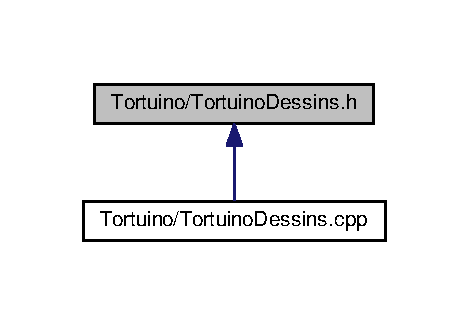
\includegraphics[width=225pt]{TortuinoDessins_8h__dep__incl}
\end{center}
\end{figure}
\subsection*{Fonctions}
\begin{DoxyCompactItemize}
\item 
void \hyperlink{TortuinoDessins_8h_afa3484b3831c738502a4c381600397ea}{triangle} (float taille\+Cote)
\begin{DoxyCompactList}\small\item\em Trace un triangle equilatéral d\textquotesingle{}une certaine taille. \end{DoxyCompactList}\item 
void \hyperlink{TortuinoDessins_8h_a8fd6d1d3aad9c0c10525e5c8244a6ce1}{carre} (float taille\+Cote)
\begin{DoxyCompactList}\small\item\em Trace un carré d\textquotesingle{}une certaine taille. \end{DoxyCompactList}\item 
void \hyperlink{TortuinoDessins_8h_ada93849cc1680d0d43bf6f9c1de954b2}{polygone\+Regulier} (int nb\+Cotes, float taille\+Cote)
\begin{DoxyCompactList}\small\item\em Fait tracer au robot un polygone régulier en fonction du nombre de côtés souhaités et de la taille de chacun de ces côtés. \end{DoxyCompactList}\item 
void \hyperlink{TortuinoDessins_8h_a57189e3fe807009b1595778589a16be9}{cercle} (float rayon)
\begin{DoxyCompactList}\small\item\em Cette fonction est une tentative de réalisation d\textquotesingle{}un cercle automatiquement avec juste le rayon souhaité en entrée. \end{DoxyCompactList}\item 
void \hyperlink{TortuinoDessins_8h_a39c1c8ca3b979edec7d841f1a71e50f1}{arbre} (int nb\+Niveaux, float taille\+Tronc)
\begin{DoxyCompactList}\small\item\em Trace un arbre récursivement dont l\textquotesingle{}angle entre les branches est de 90 degrés et qui est symétrique par rapport à l\textquotesingle{}axe formé par son tronc. \end{DoxyCompactList}\item 
void \hyperlink{TortuinoDessins_8h_ac8968b78a962de5017b660c5e8e37513}{arbre\+Symetrique} (int nb\+Niveaux, float taille\+Tronc, float angle\+Separation)
\begin{DoxyCompactList}\small\item\em Trace un arbre récursivement dont l\textquotesingle{}angle entre les branches peut être précisé et qui est symétrique par rapport à l\textquotesingle{}axe formé par son tronc. \end{DoxyCompactList}\item 
void \hyperlink{TortuinoDessins_8h_a29fa4a540a63b4e05fe0aee6d5b522c0}{arbre\+Asymetrique} (int nb\+Niveaux, float taille\+Tronc, float angle\+Separation, float angle\+Inclinaison)
\begin{DoxyCompactList}\small\item\em Trace un arbre récursivement dont l\textquotesingle{}angle entre les branches et l\textquotesingle{}angle entre la branche de gauche et la branche mère moins 45 degrés peuvent être précisés \+: il est asymétrique par rapport à l\textquotesingle{}axe formé par son tronc. \end{DoxyCompactList}\item 
void \hyperlink{TortuinoDessins_8h_a170bac7a60b14659e63b81c8eefac3dd}{sapin} (int nb\+Niveaux, float taille\+Tronc)
\begin{DoxyCompactList}\small\item\em Utilise deux arbres asymétriques pour tracer un sapin, c\textquotesingle{}est-\/à-\/dire un arbre où chaque branche se sépare en trois autres \+: une continuant vers le haut (le tronc donc) et deux horizontales sur le côté (les branches donc). \end{DoxyCompactList}\item 
void \hyperlink{TortuinoDessins_8h_af86cf0f8acc522368a052c765047a3a1}{courbe\+Von\+Koch} (int nb\+Niveaux, float taille)
\begin{DoxyCompactList}\small\item\em Trace une \href{https://fr.wikipedia.org/wiki/Flocon_de_Koch#Courbe_de_Koch}{\tt courbe de Von Koch} paramétrée par son niveau et la taille du segment de départ. \end{DoxyCompactList}\item 
void \hyperlink{TortuinoDessins_8h_afa05db28401a10aa6c4625a2de482484}{flocon} (int nb\+Niveaux, float taille)
\begin{DoxyCompactList}\small\item\em Trace un \href{https://fr.wikipedia.org/wiki/Flocon_de_Koch#Flocon_de_Koch}{\tt flocon de Von Koch} paramétré par son niveau et la taille du segment de départ. \end{DoxyCompactList}\item 
void \hyperlink{TortuinoDessins_8h_a0c851f0f43370a65c2da38436be9a764}{triangle\+Sierpinski} (int nb\+Niveaux, float taille)
\begin{DoxyCompactList}\small\item\em Trace un \href{https://fr.wikipedia.org/wiki/Triangle_de_Sierpi%C5%84ski}{\tt triangle de Sierpiński} paramétré par son niveau et la taille globale du triangle. \end{DoxyCompactList}\end{DoxyCompactItemize}


\subsection{Description détaillée}
Définition des fonctions implémentées dans \hyperlink{TortuinoDessins_8cpp}{Tortuino\+Dessins.\+cpp}. 

\begin{DoxyVersion}{Version}
1.\+1 
\end{DoxyVersion}
\begin{DoxyAuthor}{Auteur}
Paul Mabileau \href{mailto:paulmabileau@hotmail.fr}{\tt paulmabileau@hotmail.\+fr}
\end{DoxyAuthor}
Ce fichier constitue l\textquotesingle{}en-\/tête de \hyperlink{TortuinoDessins_8cpp}{Tortuino\+Dessins.\+cpp}. Il permet de préciser ce qui sera rendu accessible à d\textquotesingle{}autres programmes. Ici, ce sont des fonctions. 

\subsection{Documentation des fonctions}
\mbox{\Hypertarget{TortuinoDessins_8h_a39c1c8ca3b979edec7d841f1a71e50f1}\label{TortuinoDessins_8h_a39c1c8ca3b979edec7d841f1a71e50f1}} 
\index{Tortuino\+Dessins.\+h@{Tortuino\+Dessins.\+h}!arbre@{arbre}}
\index{arbre@{arbre}!Tortuino\+Dessins.\+h@{Tortuino\+Dessins.\+h}}
\subsubsection{\texorpdfstring{arbre()}{arbre()}}
{\footnotesize\ttfamily void arbre (\begin{DoxyParamCaption}\item[{int}]{nb\+Niveaux,  }\item[{float}]{taille\+Tronc }\end{DoxyParamCaption})}



Trace un arbre récursivement dont l\textquotesingle{}angle entre les branches est de 90 degrés et qui est symétrique par rapport à l\textquotesingle{}axe formé par son tronc. 

C\textquotesingle{}est donc un cas particulier de \hyperlink{TortuinoDessins_8cpp_ac8968b78a962de5017b660c5e8e37513}{arbre\+Symetrique(int nb\+Niveaux, float taille\+Tronc, float angle\+Separation)}.


\begin{DoxyParams}{Paramètres}
{\em nb\+Niveaux} & Le nombre de niveaux que l\textquotesingle{}arbre comprendra, c\textquotesingle{}est-\/à-\/dire le nombre de fois moins un que l\textquotesingle{}arbre va se séparer ou autrement dit la distance en nombre de branches entre la racine et chaque feuille. \\
\hline
{\em taille\+Tronc} & La taille du tronc de départ. Les branches qui en partiront auront leurs tailles d\textquotesingle{}un tier plus petites. \\
\hline
\end{DoxyParams}


Définition à la ligne 84 du fichier Tortuino\+Dessins.\+cpp.

\mbox{\Hypertarget{TortuinoDessins_8h_a29fa4a540a63b4e05fe0aee6d5b522c0}\label{TortuinoDessins_8h_a29fa4a540a63b4e05fe0aee6d5b522c0}} 
\index{Tortuino\+Dessins.\+h@{Tortuino\+Dessins.\+h}!arbre\+Asymetrique@{arbre\+Asymetrique}}
\index{arbre\+Asymetrique@{arbre\+Asymetrique}!Tortuino\+Dessins.\+h@{Tortuino\+Dessins.\+h}}
\subsubsection{\texorpdfstring{arbre\+Asymetrique()}{arbreAsymetrique()}}
{\footnotesize\ttfamily void arbre\+Asymetrique (\begin{DoxyParamCaption}\item[{int}]{nb\+Niveaux,  }\item[{float}]{taille\+Tronc,  }\item[{float}]{angle\+Separation,  }\item[{float}]{angle\+Inclinaison }\end{DoxyParamCaption})}



Trace un arbre récursivement dont l\textquotesingle{}angle entre les branches et l\textquotesingle{}angle entre la branche de gauche et la branche mère moins 45 degrés peuvent être précisés \+: il est asymétrique par rapport à l\textquotesingle{}axe formé par son tronc. 

Il généralise donc un arbre.


\begin{DoxyParams}{Paramètres}
{\em nb\+Niveaux} & Le nombre de niveaux que l\textquotesingle{}arbre comprendra, c\textquotesingle{}est-\/à-\/dire le nombre de fois moins un que l\textquotesingle{}arbre va se séparer ou autrement dit la distance en nombre de branches entre la racine et chaque feuille. \\
\hline
{\em taille\+Tronc} & La taille du tronc de départ. Les branches qui en partiront auront leurs tailles d\textquotesingle{}un tier plus petites. \\
\hline
{\em angle\+Separation} & L\textquotesingle{}angle séparant les branches provenant d\textquotesingle{}une même branche mère. \\
\hline
{\em angle\+Inclinaison} & L\textquotesingle{}angle entre la branche de gauche et la branche mère moins 45 degrés. \\
\hline
\end{DoxyParams}
\begin{DoxySeeAlso}{Voir également}
\hyperlink{TortuinoDessins_8cpp_a39c1c8ca3b979edec7d841f1a71e50f1}{arbre(int nb\+Niveaux, float taille\+Tronc)} 

\hyperlink{TortuinoDessins_8cpp_ac8968b78a962de5017b660c5e8e37513}{arbre\+Symetrique(int nb\+Niveaux, float taille\+Tronc, float angle\+Separation)} 
\end{DoxySeeAlso}


Définition à la ligne 120 du fichier Tortuino\+Dessins.\+cpp.

\mbox{\Hypertarget{TortuinoDessins_8h_ac8968b78a962de5017b660c5e8e37513}\label{TortuinoDessins_8h_ac8968b78a962de5017b660c5e8e37513}} 
\index{Tortuino\+Dessins.\+h@{Tortuino\+Dessins.\+h}!arbre\+Symetrique@{arbre\+Symetrique}}
\index{arbre\+Symetrique@{arbre\+Symetrique}!Tortuino\+Dessins.\+h@{Tortuino\+Dessins.\+h}}
\subsubsection{\texorpdfstring{arbre\+Symetrique()}{arbreSymetrique()}}
{\footnotesize\ttfamily void arbre\+Symetrique (\begin{DoxyParamCaption}\item[{int}]{nb\+Niveaux,  }\item[{float}]{taille\+Tronc,  }\item[{float}]{angle\+Separation }\end{DoxyParamCaption})}



Trace un arbre récursivement dont l\textquotesingle{}angle entre les branches peut être précisé et qui est symétrique par rapport à l\textquotesingle{}axe formé par son tronc. 

C\textquotesingle{}est donc un cas particulier de \hyperlink{TortuinoDessins_8cpp_a29fa4a540a63b4e05fe0aee6d5b522c0}{arbre\+Asymetrique(int nb\+Niveaux, float taille\+Tronc, float angle\+Separation, float angle\+Inclinaison)}.


\begin{DoxyParams}{Paramètres}
{\em nb\+Niveaux} & Le nombre de niveaux que l\textquotesingle{}arbre comprendra, c\textquotesingle{}est-\/à-\/dire le nombre de fois moins un que l\textquotesingle{}arbre va se séparer ou autrement dit la distance en nombre de branches entre la racine et chaque feuille. \\
\hline
{\em taille\+Tronc} & La taille du tronc de départ. Les branches qui en partiront auront leurs tailles d\textquotesingle{}un tier plus petites. \\
\hline
{\em angle\+Separation} & L\textquotesingle{}angle séparant les branches provenant d\textquotesingle{}une même branche mère. \\
\hline
\end{DoxyParams}
\begin{DoxySeeAlso}{Voir également}
\hyperlink{TortuinoDessins_8cpp_a39c1c8ca3b979edec7d841f1a71e50f1}{arbre(int nb\+Niveaux, float taille\+Tronc)} 
\end{DoxySeeAlso}


Définition à la ligne 101 du fichier Tortuino\+Dessins.\+cpp.

\mbox{\Hypertarget{TortuinoDessins_8h_a8fd6d1d3aad9c0c10525e5c8244a6ce1}\label{TortuinoDessins_8h_a8fd6d1d3aad9c0c10525e5c8244a6ce1}} 
\index{Tortuino\+Dessins.\+h@{Tortuino\+Dessins.\+h}!carre@{carre}}
\index{carre@{carre}!Tortuino\+Dessins.\+h@{Tortuino\+Dessins.\+h}}
\subsubsection{\texorpdfstring{carre()}{carre()}}
{\footnotesize\ttfamily void carre (\begin{DoxyParamCaption}\item[{float}]{taille\+Cote }\end{DoxyParamCaption})}



Trace un carré d\textquotesingle{}une certaine taille. 

En réalité, ce n\textquotesingle{}est qu\textquotesingle{}une adaptation de \hyperlink{TortuinoDessins_8cpp_ada93849cc1680d0d43bf6f9c1de954b2}{polygone\+Regulier(int nb\+Cotes, float taille\+Cote)} au cas particulier du carré.


\begin{DoxyParams}{Paramètres}
{\em taille\+Cote} & La taille des côtés du carré. \\
\hline
\end{DoxyParams}


Définition à la ligne 55 du fichier Tortuino\+Dessins.\+cpp.

\mbox{\Hypertarget{TortuinoDessins_8h_a57189e3fe807009b1595778589a16be9}\label{TortuinoDessins_8h_a57189e3fe807009b1595778589a16be9}} 
\index{Tortuino\+Dessins.\+h@{Tortuino\+Dessins.\+h}!cercle@{cercle}}
\index{cercle@{cercle}!Tortuino\+Dessins.\+h@{Tortuino\+Dessins.\+h}}
\subsubsection{\texorpdfstring{cercle()}{cercle()}}
{\footnotesize\ttfamily void cercle (\begin{DoxyParamCaption}\item[{float}]{rayon }\end{DoxyParamCaption})}



Cette fonction est une tentative de réalisation d\textquotesingle{}un cercle automatiquement avec juste le rayon souhaité en entrée. 

Seulement, cela ne fonctionne pas trop car il est difficile de décoréler les paramètres du robot pour pouvoir calculer les valeurs nécessaires à une approximation relativement correcte d\textquotesingle{}un cercle par un polygone régulier au grand nombre de côtés.


\begin{DoxyParams}{Paramètres}
{\em rayon} & Le rayon du cercle. \\
\hline
\end{DoxyParams}


Définition à la ligne 68 du fichier Tortuino\+Dessins.\+cpp.

\mbox{\Hypertarget{TortuinoDessins_8h_af86cf0f8acc522368a052c765047a3a1}\label{TortuinoDessins_8h_af86cf0f8acc522368a052c765047a3a1}} 
\index{Tortuino\+Dessins.\+h@{Tortuino\+Dessins.\+h}!courbe\+Von\+Koch@{courbe\+Von\+Koch}}
\index{courbe\+Von\+Koch@{courbe\+Von\+Koch}!Tortuino\+Dessins.\+h@{Tortuino\+Dessins.\+h}}
\subsubsection{\texorpdfstring{courbe\+Von\+Koch()}{courbeVonKoch()}}
{\footnotesize\ttfamily void courbe\+Von\+Koch (\begin{DoxyParamCaption}\item[{int}]{nb\+Niveaux,  }\item[{float}]{taille }\end{DoxyParamCaption})}



Trace une \href{https://fr.wikipedia.org/wiki/Flocon_de_Koch#Courbe_de_Koch}{\tt courbe de Von Koch} paramétrée par son niveau et la taille du segment de départ. 


\begin{DoxyParams}{Paramètres}
{\em nb\+Niveaux} & Le nombre de niveaux de la courbe de Von Koch, par convention 1 donne un trait seulement. \\
\hline
{\em taille} & La taille du segment à partir de laquelle l\textquotesingle{}opération récursive est itérée, c\textquotesingle{}est-\/à-\/dire que contrairement à un arbre ou un polygone tels qu\textquotesingle{}implémentés ici, ajouter plus de niveaux ou de côtés n\textquotesingle{}augmente pas la taille globale de la courbe ; autrement dit, le segment de départ sert d\textquotesingle{}étalon pour en déduire à l\textquotesingle{}avance la taille des côtés engendrés. \\
\hline
\end{DoxyParams}


Définition à la ligne 165 du fichier Tortuino\+Dessins.\+cpp.

\mbox{\Hypertarget{TortuinoDessins_8h_afa05db28401a10aa6c4625a2de482484}\label{TortuinoDessins_8h_afa05db28401a10aa6c4625a2de482484}} 
\index{Tortuino\+Dessins.\+h@{Tortuino\+Dessins.\+h}!flocon@{flocon}}
\index{flocon@{flocon}!Tortuino\+Dessins.\+h@{Tortuino\+Dessins.\+h}}
\subsubsection{\texorpdfstring{flocon()}{flocon()}}
{\footnotesize\ttfamily void flocon (\begin{DoxyParamCaption}\item[{int}]{nb\+Niveaux,  }\item[{float}]{taille }\end{DoxyParamCaption})}



Trace un \href{https://fr.wikipedia.org/wiki/Flocon_de_Koch#Flocon_de_Koch}{\tt flocon de Von Koch} paramétré par son niveau et la taille du segment de départ. 

C\textquotesingle{}est en fait une répétition de la \hyperlink{TortuinoDessins_8cpp_af86cf0f8acc522368a052c765047a3a1}{courbe\+Von\+Koch(int nb\+Niveaux, float taille)} \+: trois fois séparées par un angle intérieur de 120 degrés.


\begin{DoxyParams}{Paramètres}
{\em nb\+Niveaux} & Le nombre de niveaux du flocon de Von Koch, par convention 1 donne un triangle seulement. \\
\hline
{\em taille} & La taille du segment à partir de laquelle l\textquotesingle{}opération récursive est itérée, c\textquotesingle{}est-\/à-\/dire que contrairement à un arbre ou un polygone tels qu\textquotesingle{}implémentés ici, ajouter plus de niveaux ou de côtés n\textquotesingle{}augmente pas la taille globale du floncon ; autrement dit, le segment de départ sert d\textquotesingle{}étalon pour en déduire à l\textquotesingle{}avance la taille des côtés engendrés. \\
\hline
\end{DoxyParams}


Définition à la ligne 191 du fichier Tortuino\+Dessins.\+cpp.

\mbox{\Hypertarget{TortuinoDessins_8h_ada93849cc1680d0d43bf6f9c1de954b2}\label{TortuinoDessins_8h_ada93849cc1680d0d43bf6f9c1de954b2}} 
\index{Tortuino\+Dessins.\+h@{Tortuino\+Dessins.\+h}!polygone\+Regulier@{polygone\+Regulier}}
\index{polygone\+Regulier@{polygone\+Regulier}!Tortuino\+Dessins.\+h@{Tortuino\+Dessins.\+h}}
\subsubsection{\texorpdfstring{polygone\+Regulier()}{polygoneRegulier()}}
{\footnotesize\ttfamily void polygone\+Regulier (\begin{DoxyParamCaption}\item[{int}]{nb\+Cotes,  }\item[{float}]{taille\+Cote }\end{DoxyParamCaption})}



Fait tracer au robot un polygone régulier en fonction du nombre de côtés souhaités et de la taille de chacun de ces côtés. 

Voir l\textquotesingle{}\href{https://fr.wikipedia.org/wiki/Polygone_r%C3%A9gulier}{\tt article Wikipédia} suivant pour plus de détails sur cette figure géométrique.


\begin{DoxyParams}{Paramètres}
{\em nb\+Cotes} & Le nombre de côtés du polygone à tracer. \\
\hline
{\em taille\+Cote} & La taille de chacun des côtés. \\
\hline
\end{DoxyParams}


Définition à la ligne 30 du fichier Tortuino\+Dessins.\+cpp.

\mbox{\Hypertarget{TortuinoDessins_8h_a170bac7a60b14659e63b81c8eefac3dd}\label{TortuinoDessins_8h_a170bac7a60b14659e63b81c8eefac3dd}} 
\index{Tortuino\+Dessins.\+h@{Tortuino\+Dessins.\+h}!sapin@{sapin}}
\index{sapin@{sapin}!Tortuino\+Dessins.\+h@{Tortuino\+Dessins.\+h}}
\subsubsection{\texorpdfstring{sapin()}{sapin()}}
{\footnotesize\ttfamily void sapin (\begin{DoxyParamCaption}\item[{int}]{nb\+Niveaux,  }\item[{float}]{taille\+Tronc }\end{DoxyParamCaption})}



Utilise deux arbres asymétriques pour tracer un sapin, c\textquotesingle{}est-\/à-\/dire un arbre où chaque branche se sépare en trois autres \+: une continuant vers le haut (le tronc donc) et deux horizontales sur le côté (les branches donc). 


\begin{DoxyParams}{Paramètres}
{\em nb\+Niveaux} & Le nombre de niveaux que l\textquotesingle{}arbre comprendra, c\textquotesingle{}est-\/à-\/dire le nombre de fois moins un que l\textquotesingle{}arbre va se séparer ou autrement dit la distance en nombre de branches entre la racine et chaque feuille. \\
\hline
{\em taille\+Tronc} & La taille du tronc de départ. Les branches qui en partiront auront leurs tailles d\textquotesingle{}un tier plus petites. \\
\hline
\end{DoxyParams}
\begin{DoxySeeAlso}{Voir également}
\hyperlink{TortuinoDessins_8cpp_a39c1c8ca3b979edec7d841f1a71e50f1}{arbre(int nb\+Niveaux, float taille\+Tronc)} 
\end{DoxySeeAlso}


Définition à la ligne 150 du fichier Tortuino\+Dessins.\+cpp.

\mbox{\Hypertarget{TortuinoDessins_8h_afa3484b3831c738502a4c381600397ea}\label{TortuinoDessins_8h_afa3484b3831c738502a4c381600397ea}} 
\index{Tortuino\+Dessins.\+h@{Tortuino\+Dessins.\+h}!triangle@{triangle}}
\index{triangle@{triangle}!Tortuino\+Dessins.\+h@{Tortuino\+Dessins.\+h}}
\subsubsection{\texorpdfstring{triangle()}{triangle()}}
{\footnotesize\ttfamily void triangle (\begin{DoxyParamCaption}\item[{float}]{taille\+Cote }\end{DoxyParamCaption})}



Trace un triangle equilatéral d\textquotesingle{}une certaine taille. 

En réalité, ce n\textquotesingle{}est qu\textquotesingle{}une adaptation de \hyperlink{TortuinoDessins_8cpp_ada93849cc1680d0d43bf6f9c1de954b2}{polygone\+Regulier(int nb\+Cotes, float taille\+Cote)} au cas particulier du triangle equilatéral.


\begin{DoxyParams}{Paramètres}
{\em taille\+Cote} & La taille des côtés du triangle. \\
\hline
\end{DoxyParams}


Définition à la ligne 44 du fichier Tortuino\+Dessins.\+cpp.

\mbox{\Hypertarget{TortuinoDessins_8h_a0c851f0f43370a65c2da38436be9a764}\label{TortuinoDessins_8h_a0c851f0f43370a65c2da38436be9a764}} 
\index{Tortuino\+Dessins.\+h@{Tortuino\+Dessins.\+h}!triangle\+Sierpinski@{triangle\+Sierpinski}}
\index{triangle\+Sierpinski@{triangle\+Sierpinski}!Tortuino\+Dessins.\+h@{Tortuino\+Dessins.\+h}}
\subsubsection{\texorpdfstring{triangle\+Sierpinski()}{triangleSierpinski()}}
{\footnotesize\ttfamily void triangle\+Sierpinski (\begin{DoxyParamCaption}\item[{int}]{nb\+Niveaux,  }\item[{float}]{taille }\end{DoxyParamCaption})}



Trace un \href{https://fr.wikipedia.org/wiki/Triangle_de_Sierpi%C5%84ski}{\tt triangle de Sierpiński} paramétré par son niveau et la taille globale du triangle. 


\begin{DoxyParams}{Paramètres}
{\em nb\+Niveaux} & Le nombre de niveaux du triangle de Sierpiński. \\
\hline
{\em taille} & La taille du segment de départ qui sera conservée au fur et à mesure des itérations de l\textquotesingle{}algorithme de Sierpiński ; idem à ce que fait \hyperlink{TortuinoDessins_8cpp_afa05db28401a10aa6c4625a2de482484}{flocon(int nb\+Niveaux, float taille)} \\
\hline
\end{DoxyParams}


Définition à la ligne 206 du fichier Tortuino\+Dessins.\+cpp.


%--- End generated contents ---

% Index
\backmatter
\newpage
\phantomsection
\clearemptydoublepage
\addcontentsline{toc}{chapter}{Index}
\printindex

\end{document}
